\documentclass[letterpaper,12pt]{article}

%% Page dimensions for 1 inch margins
\setlength{\textwidth}{6.5in}
\setlength{\textheight}{9in}
\setlength{\topmargin}{-0in}
\setlength{\oddsidemargin}{0in}
\setlength{\evensidemargin}{0in} 
\setlength{\headheight}{0in}
\setlength{\headsep}{0in} 
\setlength{\hoffset}{0in}
\setlength{\voffset}{0in}

%% Graphics and math
\usepackage{graphics,graphicx,subfigure}
\usepackage{amsmath}
\usepackage{amsfonts}
\usepackage[makeroom]{cancel}

\newcommand\lsim{\mathrel{\rlap{\lower4pt\hbox{\hskip1pt$\sim$}}
        \raise1pt\hbox{$<$}}}
\newcommand\gsim{\mathrel{\rlap{\lower4pt\hbox{\hskip1pt$\sim$}}
        \raise1pt\hbox{$>$}}}

%% Bibliographic stuff

%\usepackage[numbers]{natbib}
\usepackage{natbib}
\bibliographystyle{apj}
%\setlength{\bibsep}{0.0pt}
\usepackage{courier}

\newcommand\apjl{ApJL}
\newcommand\apj{ApJ}
\newcommand\aj{AJ}
\newcommand\apjs{ApJS}
\newcommand\aap{AAP}
\newcommand\mnras{MNRAS}
\newcommand\araa{ ARA\&A }
\newcommand\nat{ Nature }

\newcommand{\beq}{\begin{equation}}
\newcommand{\eeq}{\end{equation}}

\newcommand\reye{\mathrel{Re}}
\newcommand\reym{\mathrel{Rm}}

%Use this for citing without parentheses.
\newcommand{\citei}[1]{\citeauthor{#1} \citeyear{#1}}

\begin{document}
\pagestyle{plain}
\pagenumbering{arabic}

\title{Weakly Nonlinear MRI: Notes}
\author{Susan Clark}
\maketitle
\vspace{0.2cm}

The basic setup for this investigation will follow \citet{Umurhan:2007dz}, who apply a weakly nonlinear analysis to the MRI in the shearing box approximation, in a thin-gap limit with idealized boundary conditions. We will follow a similar derivation, without the thin-gap restriction and with more realistic boundary conditions.

The shearing box (SB) approximation is one in which one considers the flow in a small box at some fiducial distance ${r_0}$ away from the center of the rotating system. This constitutes only a small portion of an accretion disk, but makes the problem more tractable, both for analytic and numerical analyses. 

My understanding is that the thin-gap limit allows one to ignore radially-dependent (``channel") modes. Channel modes are axially symmetric, linear modes, and are exact solutions of the nonlinear MRI in the SB approximation. These are the so-called ``primary MRI" modes discussed in \citet{Pessah:2010ic}. The advantage to analyzing the MRI without channel modes is that the background is steady and has a constant pressure. By widening our gap, we will complicate things because the non-constant background means that we open ourselves to parasitic modes -- modes whose growth rates depend on the amplitudes of the primary modes. In particular, the channel modes are Kelvin-Helmholtz unstable. 

%Another way to say this is that the wide gap approximation does not allow us to
In general, we cannot ignore the $\left(\textbf{u} \cdot \nabla \right) \textbf{u}$ term in the Navier-Stokes equation, which couples velocities with each other. %and thus allows the existence of parasitic modes. 
This can be seen by considering $\textbf{u}$ as a sum of discrete modes with wavenumber k:

\begin{equation}
\textbf{u} = \sum\limits_{k = 0}^{\infty}a_k e^{ikx} \, dk
\end{equation}

\noindent The Fourier transform of $\left(\textbf{u} \cdot \nabla \right) \textbf{u}$ is:

\begin{equation}
a_k \otimes i \textbf{k} \cdot a_k
\end{equation}

\noindent Clearly, each wavenumber (and its associated amplitude) depends on all other wave numbers.\\

So essentially, our approach is similar to \citet{Umurhan:2007dz}, but our setup is complementary to \citet{Pessah:2010ic}. \\

\noindent The MRI setup in \citet{Umurhan:2007dz} is as follows: 
\begin{itemize}
\item An axisymmetric channel flow with a differential rotation ${\Omega\left(r\right) \propto \Omega_0\left(\frac{r}{r_0}\right)^{-q}}$ 
\item A velocity $\textbf{V}$ = $U\left(x\right)\hat{\bf{y}}$ with a linear shear profile $U\left(x\right) = -qU_0x$
\item Constant, vertical magnetic field $\bf{\hat{B}}$ = $B_0\hat{z}$
\end{itemize}

We will use the incompressible limit ($\nabla \cdot \textbf{u}$ = $0$), which applies because we consider weak magnetic fields (magnetic energy is small compared to thermal energy). \\

\noindent \textbf{We will proceed as follows:}

\begin{itemize}
\item Linearize equations for perturbations of the form $e^{st + ik_x x + ik_z z}$. We neglect y-dependence because of axisymmetry.
\item Write linearized equations in matrix form, use SymPy to obtain dispersion relation. This is a 4th order polynomial in s.
\end{itemize}
\textit{The following five bullet points are performed in analogy to Raleigh B\'enard convection:}
\begin{itemize}
\item We want to derive an envelope (amplitude) equation, which we will do with a multiscale analysis. We choose scalings such that $s$, $k_x$, and $k_z$ in our dispersion relation come in at the same (lowest) order in the small parameter $\epsilon$. This determines the scalings for the corresponding slow variables T, X, and Y.
\item Rewrite equations in terms of quantities that depend on both fast and slow variables, in the form $u(x, y, t; X, Y, T) = A(X, Y, T)e^{i\mathbf{k} \cdot \mathbf{x}}$.
\item Expand quantities in powers of $\epsilon$.
\item Group terms by $\mathcal{O}\left(\epsilon\right)$
\item Solve successively to obtain envelope equation. We solve up to the order where a term appears that can cause saturation.\\

%\item We are only interested in marginality to the MRI, so we will take s=0. 
%\item This should allow us to isolate the most unstable mode at criticality. 


\end{itemize} 

\noindent Things to include:
\begin{itemize}
\item Derivations that I wrote out by hand (scan)
\item Nondimensionalization 
\item Multiscale analysis (in analogy to Raleigh B\'enard convection)
\item Boundary conditions
\item Amplitude functions
\item GLE
\end{itemize}

\vspace{10cm}

\textbf{Derivation of Equations} \\

An equation for the conservation of energy is easily derived assuming an ideal gas: \\

$P = \left(\gamma - 1\right)\rho e$\\

$\partial_t e + \left(\mathbf{v}\cdot \nabla\right) e + \frac{1}{\rho}P\nabla \cdot \mathbf{u} = 0$ \\

Becomes: \\

$\partial_t P + \left(\mathbf{u} \cdot \nabla\right)P + \left(\gamma -1\right)P\nabla \cdot \mathbf{u} = 0$ \\

But in our set-up, this will become formally equivalent to the incompressible limit ($\nabla \cdot \mathbf{u} \,=\, 0$). Likewise, we can write the equation for conservation of mass: \\

$\partial_t \rho + \nabla \cdot \left(\rho \mathbf{u}\right) = 0$ \\

But later on, the small shearing box approximation and the assumption that the initial density perturbation is zero will render this equation unnecessary. \\

So instead, we begin with the momentum equation: 
%\begin{equation}
\[\partial_t \mathbf{u} \, + \, \mathbf{u} \cdot \nabla \mathbf{u} \, = \, -\frac{1}{\rho}\nabla P \, - \, \nabla\Phi \, + \, \frac{1}{\rho} \left(\mathbf{J}\times\mathbf{B}\right) \, + \, \nu\nabla^2 \mathbf{u} \, - \, 2\mathbf{\Omega} \times \mathbf{u} \, - \, \mathbf{\Omega} \times \left(\mathbf{\Omega} \times \mathbf{r} \right)\]
%\end{equation}\label{momeqn}

And the induction equation:
\[\partial_t \mathbf{B} = \nabla \times \left(\mathbf{u} \times \mathbf{B}\right) + \eta\nabla^2\mathbf{B} \]

The reference frame is rotating with angular velocity $\Omega_0 \mathbf{\hat{z}}$. \\

The Coriolis term becomes: \\

$2\mathbf{\Omega} \times \mathbf{u} \, = \, 2\Omega_0 \mathbf{\hat{z}} \times \mathbf{u} \, = \, 2\Omega_0\left(\mathbf{\hat{z}} \times u_r \mathbf{\hat{r}} \, + \, \mathbf{\hat{z}} \times u_{\phi} \mathbf{\hat{\phi}}\right) \, = \, 2\Omega_0\left(v_r \mathbf{\hat{\phi}} - v_{\phi}\mathbf{\hat{r}}\right) $\\

The centrifugal term becomes: \\

$\mathbf{\Omega} \times \left(\mathbf{\Omega} \times \mathbf{r} \right) \, = \, \Omega_0 \mathbf{\hat{z}} \times \left(\Omega_0 \mathbf{\hat{z}} \times \mathbf{\hat{r}}\right) = \Omega_0^2 \mathbf{\hat{z}} \times \left(r \mathbf{\hat{\phi}}\right) \, = \, -\Omega_0^2 r \mathbf{\hat{r}}$ \\

The gravitational force per unit mass can be written: \\

$\nabla\Phi \, = \, -\frac{1}{\rho_b}\nabla P_b + r\Omega^2 \mathbf{\hat{r}}$ \\

Where $\rho_b$ and $P_b$ are the density and pressure that satisfy a barotropic relation in a steady axisymmetric solution. \\

The current density is $\mathbf{J} = \frac{2}{\beta} \nabla \times \mathbf{B}$ and thus the Lorentz force becomes: \\

$\frac{1}{\rho} \left(\mathbf{J}\times\mathbf{B}\right) = \frac{1}{4 \pi \rho} \left( \nabla \times \mathbf{B} \right) \times \mathbf{B} = - \frac{1}{8 \pi \rho}\nabla B^2 + \frac{1}{4 \pi \rho} \left(\mathbf{B} \cdot \nabla\right)\mathbf{B}$ \\

Using the identity: \\

$\left( \nabla \times \mathbf{B} \right) \times \mathbf{B} = - \mathbf{B} \times \left( \nabla \times \mathbf{B} \right) = -\nabla \left(\mathbf{B} \cdot \mathbf{B}\right) + \left(\mathbf{B} \cdot \nabla \right)\mathbf{B} + \left(\mathbf{B} \cdot \nabla \right)\mathbf{B} + \mathbf{B} \times \left(\nabla \times \mathbf{B}\right)$ \\

However, this formulation allows the magnetic pressure term to have a component parallel to the magnetic field. Clearly $\mathbf{J} \times \mathbf{B}$ is always perpendicular to the field. This will become problematic if we leave these two terms separated \-- terms will cancel in the perturbation expansion that should not. So for the time being, we retain the Lorentz force as $\frac{1}{4 \pi \rho} \left( \nabla \times \mathbf{B} \right) \times \mathbf{B}$. \\

%The initial magnetic field is a constant vertical field $\mathbf{B} = B_0 \mathbf{\hat{z}}$, and thus the magnetic pressure term becomes: \\

%$- \frac{1}{8 \pi \rho}\nabla B^2 \,= \, - \frac{1}{8 \pi \rho} \left(2 B_0 \partial_z \mathbf{B}\right) \, = \, - \frac{1}{4 \pi \rho} \left(B_0 \partial_z \mathbf{B}\right)$ \\

We now have, for the momentum equation: 

\begin{equation}
\partial_t \mathbf{u} \, + \, \mathbf{u} \cdot \nabla \mathbf{u} \, + 2\Omega_0\left(v_r \mathbf{\hat{\phi}} - v_{\phi}\mathbf{\hat{r}}\right) \, = \, - r\left(\Omega^2 - \Omega_0^2\right)\mathbf{\hat{r}} \, -\frac{1}{\rho}\nabla P \, +\frac{1}{\rho_b}\nabla P_b \,  + \, \frac{1}{4 \pi \rho} \left( \nabla \times \mathbf{B} \right) \times \mathbf{B}  \, + \, \nu\nabla^2 \mathbf{u} \,
\end{equation}

The net radial body force in the rotating frame, $r\left(\Omega^2 - \Omega_0^2\right)$, is Taylor expanded as follows: \\

$-r\left(\Omega^2 - \Omega_0^2\right) \,= \,-2 r_0 \Omega\left(r_0\right)\left(r - r_0\right)\left.\frac{\partial \Omega}{\partial r}\right|_{r_0} \,= \, -2 r_0 \Omega\left(r_0\right)\left(r - r_0\right)\frac{\Omega_0}{r_0} \left.\frac{\partial ln \Omega}{\partial ln r}\right|_{r_0} $ \\

And the definition -$\left.\frac{\partial ln \Omega}{\partial ln r}\right|_{r_0} \equiv q$ is introduced, so that the term becomes: \\

$-2 r_0 \Omega\left(r_0\right)\left(r - r_0\right)\frac{\Omega_0}{r_0} \left.\frac{\partial ln \Omega}{\partial ln r}\right|_{r_0} \, = \, 2q\Omega_0^2\left(r - r_0\right)$ \\

We now make the shearing box approximation \-- that is, we take a small region of size $\Delta$ centered on a point $\left(r = r_0, \phi = \phi_0, z=0\right)$ in our disk. The box has sides of length $\Delta$: \\

\noindent$r_0 - \frac{\Delta}{2} \le r \le r_0 + \frac{\Delta}{2}$ \\
$\phi_0 - \frac{\Delta}{2 r_0} \le \phi \le \phi_0 + \frac{\Delta}{2 r_0}$ \\
$ - \frac{\Delta}{2} \le z \le r \frac{\Delta}{2}$ \\

Where $\delta \equiv \frac{\Delta}{r_0} \ll 1 $. The box lives in a disk of vertical height $h_0$, parameterized by $\varepsilon \equiv \frac{h_0}{r_0}$. The relative scaling of $\delta$ and $\varepsilon$ determine whether we are in the small or large shearing box limit.\\

And our momentum equation now reads: 
\[\partial_t \mathbf{u} \, + \, \mathbf{u} \cdot \nabla \mathbf{u} \, + 2\Omega_0\left(u_x \mathbf{\hat{y}} - u_{y}\mathbf{\hat{x}}\right) \, = \, 2\Omega_0^2 x q \mathbf{\hat{x}} \, -\frac{1}{\rho}\nabla P \, +\frac{1}{\rho_b}\nabla P_b \,  + \, \frac{1}{4 \pi \rho} \left( \nabla \times \mathbf{B} \right) \times \mathbf{B} + \, \nu\nabla^2 \mathbf{u} \,\]

\noindent We nondimensionalize as follows (see Regev \& Umurhan 2008): \\

\noindent x, y, and z are scaled by $\Delta = \delta r_0$ \\
Velocities are scaled by $\Omega_0 r_0 \delta$ \\
Magnetic fields are scaled by $B_0$ \\
Pressure is scaled by $\varepsilon^2 \Omega_0^2 r_0^2 \rho_0$ \\ 

And we introduce the following terms:
\[\reye \equiv \frac{\Omega_0 r_0^2 \delta^2}{\nu} \reym \equiv \frac{\Omega_0 r_0^2 \delta^2}{\eta}\]

And a pseudo-plasma beta parameter: 
\[\beta \equiv \frac{\varepsilon^2\Omega_0^2r_0^2}{v_A^2} \]

Where $v_A$ is the Alfven speed, which is ${v_A}^2 = \frac{B_0^2}{\rho_0}$. \\

To make it perfectly clear, I will write this out explicitly. Dimensional quantities are denoted by a tilde superscript, and I will first rewrite the momentum equation in its dimensional quantities: \\

\[\frac{\partial \mathbf{\widetilde{u}}}{\partial \widetilde{t}} \, + \, \mathbf{\widetilde{u}} \cdot \widetilde{\nabla} \mathbf{\widetilde{u}} \, + 2\Omega_0\left(\widetilde{u_x} \mathbf{\hat{y}} - \widetilde{u_{y}}\mathbf{\hat{x}}\right) \, = \, 2\Omega_0^2 \widetilde{x} q \mathbf{\hat{x}} \, -\frac{1}{\widetilde{\rho}}\widetilde{\nabla} \widetilde{P} \, +\frac{1}{\widetilde{\rho_b}}\widetilde{\nabla} \widetilde{P_b} \,  + \, \frac{1}{4 \pi \widetilde{\rho}} \left( \widetilde{\nabla} \times \mathbf{\widetilde{B}} \right) \times \mathbf{\widetilde{B}}  \, + \, \nu \widetilde{\nabla}^2 \mathbf{\widetilde{u}} \,\]

The explicit substitutions made are as follows: \\

$\widetilde{u} = \Omega_0 r_0 \delta u$ \\

$\widetilde{x} = \delta r_0 x$ \\

$\widetilde{\nabla} = \frac{\nabla}{\delta r_0}$ \\

$\widetilde{t} = \frac{t}{\Omega_0}$ \\ 

$\widetilde{B} = B_0 B \, \,; \,  \widetilde{P} = P_0 P \, \, ; \, \widetilde{\rho} = \rho_0 \rho $ \\

The velocity scale is related to the local sound speed scale $\left(c_{s0} \equiv \sqrt{\frac{P_0}{\rho_0}}\right)$ by:\\

$v_0 = \frac{\delta}{\varepsilon} c_{s0}$ \\

And thus: $\Omega_0 r_0 \delta = \frac{\delta}{\varepsilon} \sqrt{\frac{P_0}{\rho_0}}$ \\

Why is this a reasonable choice for the pressure scaling? The disk is vertically pressure-supported. The height of the disk is determined by the sound speed and gravity. At the radius of our box, $r_0$, the vertical scale is $h_0 = c_s/\Omega_0$. Thus $\varepsilon r_0 = c_s/\Omega_0$ and $\varepsilon$ is small if the Keplerian velocity is highly supersonic. This scaling allows us to substitute out the sound speed, which is meaningless in an incompressible flow anyway. \\

Making these substitutions, the dimensionless equation becomes: \\

%\begin{equation}
$\left(\Omega_0^2 r_0 \delta\right) \partial_t \mathbf{u} \, + \, \left(\Omega_0^2 r_0 \delta\right)\mathbf{u} \cdot \nabla \mathbf{u} \,+\, \left(\Omega_0^2 r_0 \delta\right) 2 u_x \mathbf{\hat{y}} \,-\, \left(\Omega_0^2 r_0 \delta\right) 2 u_y \mathbf{\hat{x}} \, = \, \left(\Omega_0^2 r_0 \delta\right) 2 x q \mathbf{\hat{x}} \,-\, \Omega_0^2 r_0 \left(\frac{\varepsilon^2}{\delta}\right)\frac{1}{\rho} \nabla P  \,+\, \Omega_0^2 r_0 \left(\frac{\varepsilon^2}{\delta}\right)\frac{1}{\rho_b} \nabla P_b \, - \, \frac{\varepsilon^2 \Omega_0^2 r_0}{\beta \delta} \frac{1}{4 \pi \rho} \left( \nabla \times \mathbf{B} \right) \times \mathbf{B} \, + \, \nu\left(\frac{\Omega_0}{r_0 \delta}\right) \nabla^2 \mathbf{u}$ \\
%\end{equation}

Dividing out a factor of $\left(\Omega_0^2 r_0 \delta\right)$ and rewriting in terms of $\beta$ and $\reye$ yields the nondimensionalized momentum equation: \\

$\partial_t \mathbf{u} \, + \, \mathbf{u} \cdot \nabla \mathbf{u} \, + \, 2 u_x \mathbf{\hat{y}} - 2 u_y \mathbf{\hat{x}} \, = \, 2 x q \mathbf{\hat{x}} \, - \, \frac{\varepsilon^2}{\delta^2} \frac{1}{\rho} \nabla P \, + \,  \frac{\varepsilon^2}{\delta^2} \frac{1}{\rho_b} \nabla P_b \, - \, \frac{\varepsilon^2}{\delta^2} \frac{2}{\beta \rho} \left( \nabla \times \mathbf{B} \right) \times \mathbf{B} \, + \, \frac{1}{\reye} \nabla^2 \mathbf{u}$ \\

We perform the same nondimensionalization for the induction equation: \\

\[\frac{\partial \widetilde{\mathbf{B}}}{\partial \widetilde{t}} \,  = \widetilde{\nabla} \times \left(\widetilde{\mathbf{u}} \times \widetilde{\mathbf{B}}\right) + \eta\widetilde{\nabla}^2 \widetilde{\mathbf{B}} \] 

Which expands to become:

\[\frac{\partial \widetilde{\mathbf{B}}}{\partial \widetilde{t}} \, = \, \left(\widetilde{\mathbf{B}} \cdot \widetilde{\nabla} \right) \widetilde{\mathbf{u}} \, - \, \left(\widetilde{\mathbf{u}} \cdot \widetilde{\nabla} \right) \widetilde{\mathbf{B}} \, + \, \eta \widetilde{\nabla}^2\widetilde{\mathbf{B}} \] \\

After using the vector identity:

\[\nabla \times \left(\mathbf{u} \times \mathbf{B}\right) \, = \, \mathbf{u}\left(\nabla \cdot \mathbf{B}\right) \, - \, \mathbf{B}\left(\nabla \cdot \mathbf{u}\right) \, + \, \left(\mathbf{B} \cdot \nabla\right)\mathbf{u} \, - \, \left(\mathbf{u} \cdot \nabla\right)\mathbf{B} \] \\

And applying the incompressibility and solenoidal magnetic field constraints. \\

Substituting for the dimensional variables, the induction equation becomes: \\

\[\left(\Omega_0 B_0\right) \partial_t\mathbf{B} \, = \, \left(\Omega_0 B_0\right)\left(\mathbf{B} \cdot \nabla\right)\mathbf{u} \, - \, \left(\Omega_0 B_0\right)\left(\mathbf{u} \cdot \nabla \right)\mathbf{B} \, + \, \frac{\eta B_0}{\delta^2 r_0^2}\nabla^2\mathbf{B} \]

Which, after dividing by a factor of $\left(\Omega_0 B_0\right)$ and substituting in $\reym$, becomes: \\

\[\partial_t\mathbf{B} \, = \, \left(\mathbf{B} \cdot \nabla \right)\mathbf{u} \, -\, \left(\mathbf{u} \cdot \nabla \right)\mathbf{B} \, + \, \frac{1}{\reym}\nabla^2\mathbf{B} \]

We will next take perturbations with respect to the background flow. The steady solution is $\mathbf{u} = -2 q \Omega_0 \mathbf{\hat{y}}$, $P = P_b$, $\rho = \rho_b$, and $\mathbf{B} = B_0 \mathbf{\hat{z}}$, so we find perturbation solutions of the following form (1 subscripts denote perturbations): \\

$\mathbf{u} \, = \, -q \Omega_0 x \mathbf{\hat{y}} \, + \, \mathbf{u_1}$ \\

$\rho \, = \, \rho_b + \rho_1$ \\

$P \, = \, P_b \, + \, P_1$ \\

$\mathbf{B} \, = \, B_0\mathbf{\hat{z}} + \mathbf{B_1}$ \\

We will begin with the momentum equation. To make this more explicit, we write out all 3 equations (pre-perturbation): \\

$\partial_t u_x \, + \, \left(\mathbf{u} \cdot \nabla\right)u_x \, - \, 2 u_y \, = \, 2 x q \, - \, \frac{\varepsilon^2}{\delta^2} \frac{1}{\rho} \partial_x P \, + \, \frac{\varepsilon^2}{\delta^2} \frac{1}{\rho_b} \partial_x P_b \, +\, \frac{\varepsilon^2}{\delta^2} \frac{2}{\beta \rho} \left( \nabla \times \mathbf{B} \right) \times \mathbf{B} + \, \frac{1}{\reye}\nabla^2 u_x  $ \\

$\partial_t u_y \, + \, \left(\mathbf{u} \cdot \nabla\right)u_y \, + \, 2u_x =  \, - \, \frac{\varepsilon^2}{\delta^2} \frac{1}{\rho} \partial_y P \, +\, \frac{\varepsilon^2}{\delta^2} \frac{2}{\beta \rho} \left( \nabla \times \mathbf{B} \right) \times \mathbf{B} \, + \, \frac{1}{\reye}\nabla^2 u_y  $ \\

$\partial_t u_z \, + \, \left(\mathbf{u} \cdot \nabla\right)u_z \,  =  \, - \, \frac{\varepsilon^2}{\delta^2} \frac{1}{\rho} \partial_z P \,  + \, \frac{\varepsilon^2}{\delta^2} \frac{1}{\rho_b} \partial_z P_b \, +\, \frac{\varepsilon^2}{\delta^2} \frac{2}{\beta \rho} \left( \nabla \times \mathbf{B} \right) \times \mathbf{B} \, + \, \frac{1}{\reye}\nabla^2 u_z $ \\

Where we have made the substitution $\partial_y P_b = \partial_y \rho_b = 0$, as the steady barotropic solution must be axisymmetric. \\

The term $\left(\mathbf{u} \cdot \nabla\right)\mathbf{u}$ expands as follows:\\

$\left(-q \Omega_0 x \mathbf{\hat{y}} \, + \, \mathbf{u_1}\right) \cdot \nabla \left(-q \Omega_0 x \mathbf{\hat{y}} \, + \, \mathbf{u_1}\right) \, = \, - q \Omega_0 x \mathbf{\hat{y}} \cdot \nabla \mathbf{u_1} + \mathbf{u_1} \cdot \nabla \mathbf{u_1} \, = \, - q \Omega_0 x \partial_y \mathbf{u_1} + \mathbf{u_1} \cdot \nabla \mathbf{u_1}$ \\

Because all of the $\nabla \left(-q \Omega_0 x \mathbf{\hat{y}}\right)$ terms are 0. \\

%Similarly, the magnetic tension term expands to become: \\

%$\left(\mathbf{B} \cdot \nabla \right)\mathbf{B} \, = \, \left(\left(B_0 \mathbf{\hat{z}} + \mathbf{B_1} \right)\cdot \nabla \right)\left(B_0 \mathbf{\hat{z}} + \mathbf{B_1} \right) \, = \, B_0 \partial_z \mathbf{B_1} \, + \, \mathbf{B_1} \cdot \nabla \mathbf{B_1}$ \\

%Because the $\nabla B_0 \mathbf{\hat{z}}$ terms are 0.

%The magnetic pressure term expands to become: \\

%$\nabla \left(B_0 \mathbf{\hat{z}} + \mathbf{B_1}\right)^2 $ \\

The Lorentz force term $\frac{\varepsilon^2}{\delta^2} \frac{2}{\beta \rho} \left( \nabla \times \mathbf{B} \right) \times \mathbf{B}$ expands as follows: \\

$ \left( \nabla \times \left(B_0 \mathbf{\hat{z}} + \mathbf{B_1}\right) \right) \times \left(B_0 \mathbf{\hat{z}} + \mathbf{B_1}\right) \, = \, \left( \nabla \times B_0 \mathbf{\hat{z}} + \nabla \times \mathbf{B_1} \right) \times \left(B_0 \mathbf{\hat{z}} + \mathbf{B_1}\right) \, $ \\

$= \, \left( \nabla \times B_0 \mathbf{\hat{z}} + \nabla \times \mathbf{B_1} \right) \times B_0 \mathbf{\hat{z}} + \left( \nabla \times B_0 \mathbf{\hat{z}} + \nabla \times \mathbf{B_1} \right) \times \mathbf{B_1} \, $ \\

$= \, \nabla \times B_0 \mathbf{\hat{z}} \times B_0 \mathbf{\hat{z}} \, +\, \nabla \times \mathbf{B_1} \times B_0 \mathbf{\hat{z}} \, + \, \nabla \times B_0 \mathbf{\hat{z}} \times \mathbf{B_1} \, + \, \nabla \times \mathbf{B_1} \times \mathbf{B_1}$\\

$= \, -\frac{\nabla B_0^2}{2} \, + \, B_0 \mathbf{\hat{z}} \cdot \nabla \left(B_0 \mathbf{\hat{z}}\right) \, - \, \nabla\left(B_0 \mathbf{\hat{z}} \cdot \mathbf{B_1}\right) \, + \, B_0 \mathbf{\hat{z}} \cdot \nabla \mathbf{B_1} \, + \, \mathbf{B_1} \cdot \nabla B_0 \mathbf{\hat{z}} \, + \, \mathbf{B_1} \times \nabla \times B_0 \mathbf{\hat{z}} \, + \, \nabla \times B_0 \mathbf{\hat{z}} \times \mathbf{B_1} \, - \, \frac{\nabla \mathbf{B_1}^2}{2} \, + \, \mathbf{B_1} \cdot \nabla \mathbf{B_1}$ \\

Now the $\nabla B_0 \mathbf{\hat{z}}$ terms are zero, and $\mathbf{B_1} \times \nabla \times B_0 \mathbf{\hat{z}} \, = \, - \nabla \times B_0 \mathbf{\hat{z}} \times \mathbf{B_1}$, so those two terms cancel one another. So we have: \\

$ = \, \frac{\varepsilon^2}{\delta^2} \frac{1}{\beta} \frac{1}{4 \pi \rho} \left(-\frac{\nabla B_0^2}{2} \, - \, \nabla \left(B_0 \mathbf{\hat{z}}\cdot \mathbf{B_1}\right)\, + \, B_0 \mathbf{\hat{z}} \cdot \nabla \mathbf{B_1} \, - \, \frac{\nabla \mathbf{B_1}^2}{2} \, + \, \mathbf{B_1}\cdot \nabla \mathbf{B_1} \, \right)$ \\

$ = \, \frac{\varepsilon^2}{\delta^2} \frac{1}{\beta} \frac{1}{4 \pi \rho} \left(-\frac{\nabla B_0^2}{2} \, - \, B_0 \mathbf{\hat{z}} \cdot \nabla \mathbf{B_1} \, + \, B_0 \cdot \nabla \mathbf{B_1} \,+ \, B_0 \mathbf{\hat{z}} \cdot \nabla \mathbf{B_1} \, - \, \frac{\nabla\mathbf{B_1}^2}{2} \, + \, \mathbf{B_1}\cdot \nabla \mathbf{B_1} \, \right)$ \\

And finally, the Lorentz force term becomes: \\

$\frac{\varepsilon^2}{\delta^2} \frac{1}{\beta} \frac{1}{4 \pi \rho} \left( \nabla \times \mathbf{B} \right) \times \mathbf{B} \, = \, \frac{\varepsilon^2}{\delta^2} \frac{1}{\beta} \frac{1}{4 \pi \rho} \left(B_0 \mathbf{\hat{z}} \cdot \nabla \mathbf{B_1} - \, \frac{\nabla \mathbf{B_1}^2}{2} \, + \, \mathbf{B_1}\cdot \nabla \mathbf{B_1} \, \right)$ \\

Which simplifies to: \\

$\frac{\varepsilon^2}{\delta^2} \frac{1}{\beta} \frac{1}{4 \pi \rho} \left( \nabla \times \mathbf{B} \right) \times \mathbf{B} \, = \, \frac{\varepsilon^2}{\delta^2} \frac{1}{\beta} \frac{1}{4 \pi \rho} \left(B_0 \partial_z \mathbf{B_1} - \, \frac{\nabla \mathbf{B_1}^2}{2} \, + \, \mathbf{B_1}\cdot \nabla \mathbf{B_1} \, \right)$ \\

The three momentum equations become: \\

$\partial_t u_{1x} \, - \, q \Omega_0 x \partial_y u_{1x} \,+ \, \left(\mathbf{u_1} \cdot \nabla\right)u_{1x} \, + \, 2 q \Omega_0 x \, - \, 2 u_{1y}\,= \, 2 q x \, - \, \frac{\varepsilon^2}{\delta^2} \left( \frac{\partial_x P_1}{\rho_1 + \rho_b} - \frac{\rho_1\partial_x P_b}{\rho_b^2 + \rho_1\rho_b}\right) \, + \frac{\varepsilon^2}{\delta^2} \frac{1}{\beta} \frac{2}{\beta} \frac{1}{\rho_b + \rho} \left( B_0 \partial_z B_{1x} \,- \, \frac{\nabla B_{1x}^2}{2} \, + \, \mathbf{B_1}\cdot \nabla B_{1x} \right) \, + \, \frac{1}{\reye}\nabla^2 u_x  $ \\

$\partial_t u_{1y} \, - \, q \Omega_0 u_{1x} \, - \, q \Omega_0 x \partial_y u_{1y} \,+ \, \left(\mathbf{u_1} \cdot \nabla\right)u_{1y} \,+ \, 2u_{1x} \, =  $\\
$\, - \, \frac{\varepsilon^2}{\delta^2} \left( \frac{\partial_y P_1}{\rho_1 + \rho_b} \right) \, + \, \frac{\varepsilon^2}{\delta^2} \frac{1}{\beta} \frac{2}{\beta} \frac{1}{\rho_b + \rho} \left( B_0 \partial_z B_{1y} \,- \, \frac{\nabla B_{1y}^2}{2} \, + \, \mathbf{B_1}\cdot \nabla B_{1y} \right) \, + \, \frac{1}{\reye}\nabla^2 u_y  $ \\

$\partial_t u_{1z} \, - \, q \Omega_0 x \partial_y u_{1z} \,+ \, \left(\mathbf{u_1} \cdot \nabla\right)u_{1z} \, = $\\
$\, - \, \frac{\varepsilon^2}{\delta^2} \left( \frac{\partial_z P_1}{\rho_1 + \rho_b} - \frac{\rho_1\partial_z P_b}{\rho_b^2 + \rho_1\rho_b}\right) \, + \frac{\varepsilon^2}{\delta^2} \frac{1}{\beta} \frac{2}{\beta} \frac{1}{\rho_b + \rho} \left( B_0 \partial_z B_{1z} \,- \, \frac{\nabla B_{1z}^2}{2} \, + \, \mathbf{B_1}\cdot \nabla B_{1z} \right) \, + \, \frac{1}{\reye}\nabla^2 u_x  $ \\

In the small shearing box (SSB) limit, $\delta \ll \varepsilon \ll 1$. For a rotation law that is close to Keplerian, $\frac{1}{\rho_b}\partial_xP_b = \mathcal{O}\left(\delta^3/\varepsilon^2\right). $

The following replacements are made: \\

\noindent $\partial_i P_b$ becomes $\frac{\delta^2}{\varepsilon^2} \partial_i P_b $ \\
$\partial_i \rho_b$ becomes $\frac{\delta^2}{\varepsilon^2} \partial_i \rho_b $ \\

The pressure perturbation can be expanded: \\

$P_1 = P_0 + \frac{\delta^2}{\varepsilon^2}\partial_i p$ where $P_0$ is a constant that gets absorbed into $P_b$. \\

This is equivalent to taking $\delta = \varepsilon^2$. Making these substitutions and taking $\rho_1 = 0$, we obtain: \\

$\partial_t u_{1x} \, - \, q \Omega_0 x \partial_y u_{1x} \,+ \, \left(\mathbf{u_1} \cdot \nabla\right)u_{1x} \, - \, 2 u_{1y}\,= \, - \, \frac{1}{\rho_b}\partial_x p  \, + \frac{1}{\beta} \frac{2}{\beta} \frac{1}{\rho_b} \left( B_0 \partial_z B_{1x} \,- \, \frac{\nabla B_{1x}^2}{2} \, + \, \mathbf{B_1}\cdot \nabla B_{1x} \right) \, + \, \frac{1}{\reye}\nabla^2 u_x  $ \\

$\partial_t u_{1y}\, - \, q \Omega_0 u_{1x}  \, - \, q \Omega_0 x \partial_y u_{1y} \,+ \, \left(\mathbf{u_1} \cdot \nabla\right)u_{1y} \,+ \, 2u_{1x} \, =  $\\
$\, - \, \frac{1}{\rho_b}\partial_y p \, + \,  \frac{1}{\beta} \frac{2}{\beta} \frac{1}{\rho_b} \left( B_0 \partial_z B_{1y} \,- \, \frac{\nabla B_{1y}^2}{2} \, + \, \mathbf{B_1}\cdot \nabla B_{1y} \right) \, + \, \frac{1}{\reye}\nabla^2 u_y  $ \\

$\partial_t u_{1z} \, - \, q \Omega_0 x \partial_y u_{1z} \,+ \, \left(\mathbf{u_1} \cdot \nabla\right)u_{1z} \, = \, - \, \frac{1}{\rho_b}\partial_z p  \, + \frac{1}{\beta} \frac{2}{\beta} \frac{1}{\rho_b} \left( B_0 \partial_z B_{1z} \,- \, \frac{\nabla B_{1z}^2}{2} \, + \, \mathbf{B_1}\cdot \nabla B_{1z} \right) \, + \, \frac{1}{\reye}\nabla^2 u_x  $ \\

Now we reparameterize in terms of the total (gas and magnetic) pressure: \\

$\Pi \equiv p + \frac{1}{2\beta} B^2$ \\

And take $\rho_b$ = 1. And finally, we have the perturbed, nondimensionalized momentum equation in all its glory: \\

$\partial_t \mathbf{u_1} \, - \, q\Omega_0 x \partial_y \mathbf{u_1} \, + \, \left(\mathbf{u_1}\cdot \nabla\right) \mathbf{u_1} \, - \, 2 u_{1y} \mathbf{\hat{x}} \, + \, \left(2 - \Omega_0 q\right)u_{1x}\mathbf{\hat{y}} \, = \, \frac{2}{\beta} \nabla \Pi \, + \, \frac{2}{\beta}B_0\partial_z\mathbf{B_1} \, + \, \frac{2}{\beta}\mathbf{B_1} \cdot \nabla \mathbf{B_1} \,+ \, \frac{1}{\reye}\nabla^2 \mathbf{u_1}$ \\

We now formally show what happens to the energy equation. If we perform the same steps as above on our energy equation: \\

$\frac{\partial}{\partial\widetilde{t}} \widetilde{P} + \left(\widetilde{\mathbf{u}} \cdot \widetilde{\nabla} \right)\widetilde{P} + \left(\gamma -1\right)\widetilde{P} \widetilde{\nabla} \cdot \widetilde{\mathbf{u}} = 0$ \\

That is, nondimensionalize: \\

$\Omega_0^3 r_0^2 \varepsilon^2 \rho_0 \frac{\partial}{\partial t} P \, + \, \Omega_0^3 r_0^2 \varepsilon^2 \rho_0 \left(\mathbf{u} \cdot \nabla \right) P \, + \, \Omega_0^3 r_0^2 \varepsilon^2 \rho_0 \left(\gamma - 1 \right) P \nabla \cdot \mathbf{u} \, = \, 0 $ \\

$\partial_t P \, + \, \left(\mathbf{u} \cdot \nabla \right) P \, + \, \left(\gamma - 1 \right) P \nabla \cdot \mathbf{u} \, = \, 0 $ \\

Take perturbations: \\

$\partial_t P_1 \, - \, q\Omega_0 x \partial_y P_1 \, + \, u_{1x}\partial_x P_b \, + \, u_{z1}\partial_z P_b \, + \, \left(\gamma - 1 \right) P_b \nabla \cdot \mathbf{u_1} \, + \, \mathbf{u_1} \cdot \nabla P_1 \, \, + \, \left(\gamma - 1\right)P_1 \nabla \cdot \mathbf{u_1} \, = \, 0$ \\

Substitute in $P_1 = \frac{\delta^2}{\varepsilon^2} p$ and $\partial_i \rho_b$ = $\frac{\delta^2}{\varepsilon^2} \partial_i \rho_b$ and $\partial_i P_b$ = $\frac{\delta^2}{\varepsilon^2} \partial_i P_b$: \\

$\frac{\delta^2}{\varepsilon^2}\partial_t p \, - \, \frac{\delta^2}{\varepsilon^2}q\Omega_0 x \partial_y p \, + \, \frac{\delta^2}{\varepsilon^2}u_{1x}\partial_x P_b \, + \, \frac{\delta^2}{\varepsilon^2}u_{z1}\partial_z P_b \, + \, \left(\gamma - 1 \right) P_b \nabla \cdot \mathbf{u_1} \, + \, \frac{\delta^2}{\varepsilon^2}\mathbf{u_1} \cdot \nabla p \, \, + \, \frac{\delta^2}{\varepsilon^2}\left(\gamma - 1\right)p \nabla \cdot \mathbf{u_1} \, = \, 0$ \\

Drop terms of $\mathcal{O}\left(\frac{\delta^2}{\varepsilon^2}\right)$, and we recover:\\

$\nabla \cdot \mathbf{u_1} \, = \, 0$ \\

Thus we have formally proven that we are working in the incompressible limit! \\

As for the induction equation, we already nondimensionalized to obtain: \\

$\partial_t\mathbf{B} \, = \, \left(\mathbf{B} \cdot \nabla \right)\mathbf{u} \, -\, \left(\mathbf{u} \cdot \nabla \right)\mathbf{B} \, + \, \frac{1}{\reym}\nabla^2\mathbf{B} $ \\

%If we plug in perturbations and all terms involving $\nabla\left(-q\Omega_0 x \mathbf{\hat{y}}\right)$ or $\nabla B_0 \mathbf{\hat{z}}$ go to zero, we arrive at: \\

For the first two terms on the righthand side, plugging in perturbations yields: \\

$\left(\mathbf{B} \cdot \nabla \right)\mathbf{u} \, -\, \left(\mathbf{u} \cdot \nabla \right)\mathbf{B} \, = \, \left(B_0 \mathbf{\hat{z}} + \mathbf{B_1}\right)\cdot\nabla \left(-q\Omega_0 x \mathbf{\hat{y}} + \mathbf{u_1}\right) \, - \, \left(-q\Omega_0 x \mathbf{\hat{y}} + \mathbf{u_1}\right) \cdot \nabla \left(B_0 \mathbf{\hat{z}} + \mathbf{B_1}\right) $ \\

$ = B_0 \partial_z \mathbf{u_1} \, + \, \mathbf{B_1}\cdot\nabla\mathbf{u_1} \, + \, q \Omega_0 x \partial_y \mathbf{B_1} \, - \, \mathbf{u_1}\cdot\nabla\mathbf{B_1} \, + \, \mathbf{B_1}\cdot \nabla\left(-q\Omega_0x \mathbf{\hat{y}}\right) \, + \, B_0\mathbf{\hat{z}} \cdot \nabla\left(-q\Omega_0x \mathbf{\hat{y}}\right) $ \\

Because all terms with $\nabla B_0 \mathbf{\hat{z}}$ go to zero. That last term goes to zero, and the term $\mathbf{B_1}\cdot \nabla\left(-q\Omega_0x \mathbf{\hat{y}}\right) \, = \, B_{1x} \partial_x\left(-q \Omega_0 x \right) \mathbf{\hat{y}}$ \\

So the induction equation becomes: \\

$\partial_t \mathbf{B_1} \, = \, B_0 \partial_z \mathbf{u_1} \, + \, \mathbf{B_1} \cdot \nabla \mathbf{u_1} \, + \, q \Omega_0 x \partial_y \mathbf{B_1} \, - \, \mathbf{u_1} \cdot \nabla \mathbf{B_1} \, - \, q\Omega_0 B_{1x} \mathbf{\hat{y}} \,+ \, \frac{1}{\reym} \nabla^2 \mathbf{B_1} $ \\

And finally we have our full equation set: \\

$\partial_t \mathbf{u_1} \, - \, q\Omega_0 x \partial_y \mathbf{u_1} \, + \, \left(\mathbf{u_1}\cdot \nabla\right) \mathbf{u_1} \, - \, 2 u_{1y} \mathbf{\hat{x}} \, + \, \left(2 - \Omega_0 q\right)u_{1x}\mathbf{\hat{y}} \, = \, \frac{2}{\beta} \nabla \Pi \, + \, \frac{2}{\beta}B_0\partial_z\mathbf{B_1} \, + \, \frac{2}{\beta}\mathbf{B_1} \cdot \nabla \mathbf{B_1}\,  + \, \frac{1}{\reye}\nabla^2 \mathbf{u_1}$ \\

$\partial_t \mathbf{B_1} \, = \, B_0 \partial_z \mathbf{u_1} \, + \, \mathbf{B_1} \cdot \nabla \mathbf{u_1} \, + \, q \Omega_0 x \partial_y \mathbf{B_1} \, - \, \mathbf{u_1} \cdot \nabla \mathbf{B_1} \, - \, q\Omega_0 B_{1x} \mathbf{\hat{y}} \,\, + \, \frac{1}{\reym} \nabla^2 \mathbf{B_1} $ \\

$\nabla \cdot \mathbf{u_1} \, = \, 0$\\

$\nabla \cdot \mathbf{B_1} \, = \, 0$ \\ 

\section*{Streamfunctions}

Because we are working with a flow that is axisymmetric and incompressible, we can reparameterize the velocity in terms of its streamfunction. \\

We express the velocity perturbation in terms of the curl of some vector field $\Psi$: \\
 
 $\mathbf{u_1} \, = - \, \nabla \times \Psi\left(x, z\right) \mathbf{\hat{y}}$ \\
 
 This expands as follows: \\
 
 $- \nabla \times \Psi\left(x, z\right) \mathbf{\hat{y}} \, = \, - \Psi\nabla \times \mathbf{\hat{y}} \, + \, \mathbf{\hat{y}} \times \nabla \Psi \, = \, \mathbf{\hat{y}} \times \nabla \Psi \,$ \\
 
 $= \, \mathbf{\hat{y}} \times \partial_x \Psi \mathbf{\hat{x}} \, + \, \mathbf{\hat{y}} \times \partial_z \Psi \mathbf{\hat{z}} \, = \, -\partial_x \Psi \mathbf{\hat{z}} \, + \, \partial_z \Psi \mathbf{\hat{x}}$ \\
 
 And thus we have: \\
 
$u_{x1} = \partial_z \Psi$ \, and \, $u_{z1} = -\partial_x \Psi$ \\

We can check that this works in the following way. Expanding the incompressibility requirement, we have: \\

$\nabla \cdot \mathbf{u_1} \, = \, \partial_x u_{1x} \, \, + \partial_z u_{1z} \, = \, 0$ \\

Because the $\partial_y$ term is 0 even if $u_{1y}$ itself is nonzero. So we see that we can enforce this requirement if we rewrite the velocity in terms of a function $\Psi$ such that:\\

$u_{x1} \, = \, \frac{\partial \Psi}{\partial z}$ \, \, and \, \, $u_{z1} \, = \, - \frac{\partial \Psi}{\partial x}$ \\

Because, plugging into the incompressibility condition: \\

\[\frac{\partial \left(\frac{\partial \Psi}{\partial z}\right)}{\partial x} \, + \, \frac{\partial \left(- \frac{\partial \Psi}{\partial x}\right)}{\partial z} \, = \, \frac{\partial^2 \Psi}{\partial x \partial z} \, - \, \frac{\partial^2 \Psi}{\partial x \partial z} \, = \, 0\] \\

This is clearly zero always. Thus, we have the stream function $\Psi$, defined such that $\left(u_{x1}, u_{z1}\right) \, = \, \left(\partial_z \Psi, -\partial_x \Psi\right)$. Analogously, we can use the solenoidal magnetic field constraint $\nabla \cdot \mathbf{B_1} \, = \, 0$ to define a flux function based on the vector potential A: \\

$B_{1x} = \partial_z A$ \, and \, $B_{1z} = - \partial_x A$ \\

Essentially, we plug in the following to our equations: \\

$\mathbf{B_1} \, = \, \left(\begin{matrix}

\partial_zA \\
B_{1y} \\
-\partial_xA \\

\end{matrix}\right)$ \, and \, $\mathbf{u_1} \, = \, \left(\begin{matrix}

\partial_z\Psi \\
u_{1y} \\
-\partial_x\Psi \\
\end{matrix}\right)$ \\

For the x component of the momentum equation, we have: \\

$\partial_t u_{1x} \, - \, q \Omega_0 x \partial_y u_{1x} \, + \, \left(\mathbf{u_1} \cdot \nabla\right) u_{1x} \, - \, 2 u_{1y} \, = \, \frac{2}{\beta} \partial_x \Pi \, + \, \frac{2}{\beta} B_0 \partial_z B_{1x} \, + \, \frac{2}{\beta} \mathbf{B_1} \cdot \nabla B_{1x} \, + \, \frac{1}{\reye}\nabla^2 u_{1x} $ \\

The $\partial_y$ terms go to zero, and this expands to become: \\

$\partial_t\partial_z\Psi \, + \, \partial_z\Psi \partial_x \partial_z \Psi \, - \, \partial_x \Psi \partial_z^2\Psi \, - \, 2 u_{1y} \, = \, \frac{2}{\beta}\partial_x \Pi \, + \, \frac{2}{\beta} B_0 \partial_z^2 A \, + \, \frac{2}{\beta} \partial_z A \partial_x \partial_z A \, - \, \frac{2}{\beta} \partial_x A \partial_z^2 A \, + \, \frac{1}{\reye} \nabla^2 \partial_z \Psi$ \\

Multiplying through by $\partial_z$ and expanding terms yields: \\

$\partial_t \partial_z^2 \Psi \, + \, \partial_z^2\Psi\partial_x\partial_z\Psi \, + \, \partial_z\Psi \partial_x\partial_z^2 \Psi \, - \, \partial_z\partial_x\Psi\partial_z^2\Psi \, - \, \partial_x \Psi \partial_z^3 \Psi \, - \, 2\partial_z u_{1y} \, = \, \frac{2}{\beta}\partial_z\partial_x\Pi \, + \, \frac{2}{\beta} B_0\partial_z^3A \, + \, \frac{2}{\beta}\partial_z^2 A \partial_x \partial_z A \, + \, \frac{2}{\beta}\partial_zA\partial_x\partial_z^2 A \, - \, \frac{2}{\beta}\partial_z\partial_x A \partial_z^2 A \, - \, \frac{2}{\beta}\partial_xA\partial_z^3A \, + \, \frac{1}{\reye} \nabla^2 \partial_z^2 \Psi $ \\

Several terms cancel, and several can be grouped into Jacobians: \\

$J\left(\Psi, \partial_z^2\Psi\right) \, = \, \partial_z \Psi \partial_x\partial_z^2\Psi \, - \, \partial_x\Psi\partial_z^3\Psi $ \\

$J\left(A, \partial_z^2 A\right) \, = \, \partial_z A \partial_x\partial_z^2A \, - \, \partial_xA\partial_z^3A $

Where $J\left(f, g\right) \equiv \partial_z f \partial_x g - \partial_x f \partial_z g$ \\ 

The x-component of the momentum equation then becomes: \\

$\partial_t\partial_z^2\Psi \, + \, J\left(\Psi, \partial_z^2\Psi\right) \, - \, 2\partial_z u_{1y} \, = \, \frac{2}{\beta}\partial_x\partial_z\Pi \, + \, \frac{2}{\beta}B_0 \partial_z^3A \, + \, \frac{2}{\beta}J\left(A, \partial_z^2A\right) \, + \, \frac{1}{\reye}\nabla^2 \partial_z^2 \Psi$ \\

The z-component of the momentum equation is: \\

$\partial_t u_{1z} \, - \, q\Omega_0x\partial_y u_{1z} \, + \, \left(\mathbf{u_1} \cdot \nabla \right) u_{1z} \, = \, \frac{2}{\beta}\partial_z \Pi \, + \, \frac{2}{\beta} B_0 \partial_z\partial_zB_{1z} \, + \, \frac{2}{\beta}\mathbf{B_1}\cdot\nabla B_{1z} \, + \, \frac{1}{\reye}\nabla^2 u_{1z} $ \\

Which, after following the steps outlined above in the expansion of the x-component, becomes: \\

$\partial_t \partial_x^2 \Psi \, + \, J\left(\Psi, \partial_x^2 \Psi\right) \, = \, -\frac{2}{\beta}\partial_x\partial_z\Pi \, + \, \frac{2}{\beta}B_0\partial_z\partial_x^2 A \, + \, \frac{2}{\beta}J\left(A, \partial_x^2 A \right) \, + \, \frac{1}{\reye} \nabla^2 \partial_x^2 \Psi$ \\

We can combine the two equations (for the x- and z-components), noting that: \\

$\nabla^2 \, = \, \partial_x^2 \mathbf{\hat{x}} \, \partial_z^2 \mathbf{\hat{z}}$ \\

$\partial_t \nabla^2 \Psi \, + \, J\left(\Psi, \nabla^2 \Psi\right) \, - \, 2 \partial_z u_{1y} \, = \, \frac{2}{\beta} B_0 \partial_z \nabla^2 A \, + \, \frac{2}{\beta}J\left(A, \nabla^2 A \right) \, + \, \frac{1}{\reye}\nabla^4 \Psi$ \\

Where the term $\frac{2}{\beta}\partial_x\partial_z\Pi \left(\mathbf{\hat{x}} \, - \, \mathbf{\hat{z}}\right)$ goes to zero. \\

The y-component of the momentum equation is even simpler: \\

$\partial_t u_{1y} \, - q\Omega_0 x \partial_y u_{1y} \, + \, \left(\mathbf{u_1} \cdot \nabla \right)u_{1y} \, + \, \left(2 - \Omega_0 q\right) u_{1x} \, = \, \frac{2}{\beta} \partial_y \Pi \, + \, \frac{2}{\beta} B_0 \partial_z B_{1y} \, + \, \frac{2}{\beta}\mathbf{B_1} \cdot \nabla B_{1y} \, + \, \frac{1}{\reye}\nabla^2 u_{1y}$ \\

Which becomes: \\

$\partial_t u_{1y} \, + \, J\left(\Psi, u_{1y}\right) \, + \, \left(2 - \Omega_0 q\right) \partial_z \Psi \, = \, \frac{2}{\beta}B_0\partial_z B_{1y} \, + \, \frac{2}{\beta} J\left(A, B_{1y}\right) \, + \, \frac{1}{\reye} \nabla^2 u_{1y}$ \\


For the induction equation, we begin with the y component: \\

$\partial_t B_{1y} \, = \, B_0 \partial_z u_{1y} \, + \, \mathbf{B_1} \cdot \nabla u_{1y} \, + \, q \Omega_0x\partial_y B_{1y} \, - \, \mathbf{u_1} \cdot \nabla B_{1y} \, + \, \frac{1}{\reym} \nabla^2 B_{1y} \, - \, q\Omega_0 B_{1x} \,$ \\

Where: \\

$\nabla u_{1y} \, = \, \partial_x u_{1y} \mathbf{\hat{x}} \, + \, \partial_z u_{1y}\mathbf{\hat{z}}$ \\

$\nabla B_{1y} \, = \, \partial_x B_{1y}\mathbf{\hat{x}} \, + \, \partial_z B_{1y}\mathbf{\hat{z}}$ \\

The equation expands to become: \\

$\partial_t B_{1y} \, = \, B_0 \partial_z u_{1y} \, + \, \partial_z A \mathbf{\hat{x}} \cdot \partial_x u_{1y}\mathbf{\hat{x}} \, + \, \partial_z A \mathbf{\hat{x}} \cdot \partial_z u_{1y} \mathbf{\hat{z}} \, - \, \partial_x A \mathbf{\hat{z}} \cdot \partial_x u_{1y} \mathbf{\hat{x}} \, - \, \partial_x A \mathbf{\hat{z}} \cdot \partial_z u_{1y} \mathbf{\hat{z}} \, + \, B_{1y}\mathbf{\hat{y}} \cdot \partial_x u_{1y} \mathbf{\hat{x}} \, + \, B_{1y}\mathbf{\hat{y}} \cdot \partial_z u_{1y} \mathbf{\hat{z}} \, + \, q\Omega_0 x \partial_y B_{1y} \mathbf{\hat{y}} \, - \, \partial_z\Psi\mathbf{\hat{x}}\cdot \partial_x B_{1y} \mathbf{\hat{x}} \, - \, \partial_z\Psi\mathbf{\hat{x}}\cdot \partial_z B_{1y} \mathbf{\hat{z}} \, + \, \partial_x\Psi\mathbf{\hat{z}}\cdot \partial_x B_{1y} \mathbf{\hat{x}} \, + \, \partial_x\Psi\mathbf{\hat{z}}\cdot \partial_z B_{1y} \mathbf{\hat{z}} \, - \, u_{1y} \mathbf{\hat{y}} \partial_x B_{1y} \mathbf{\hat{x}} \, - \, u_{1y}\mathbf{\hat{y}} \partial_z B_{1y} \mathbf{\hat{z}} \, + \, \frac{1}{\reym} \nabla^2 B_{1y} \, - \, q\Omega_0 \left(\partial_z A \right)$ \\

Clearly most of these terms cancel in the dot product, and we are left with: \\

$\partial_t B_{1y} \, = \, B_0 \partial_z u_{1y} \, + \, \partial_z A \partial_x u_{1y} \, - \, \partial_x A \partial_z u_{1y} \, + \, q\Omega_0 x \partial_y B_{1y} \, - \, \partial_z\Psi \partial_x B_{1y} \, + \, \partial_x\Psi \partial_z B_{1y} \, + \, \frac{1}{\reym} \nabla^2 B_{1y} \, - \, q \Omega_0 \partial_z A$ \\

The nonlinear terms are Jacobians, and $\partial_y B_{1y} = 0$: \\

$\partial_t B_{1y} \, = \, B_0 \partial_z u_{1y} \, + \, J\left(A, u_{1y}\right) \, - \, J\left(\Psi, B_{1y}\right) \, + \, \frac{1}{\reym} \nabla^2 B_{1y}  \, - \, q \Omega_0 \partial_z A$ \\

The x component of the induction equation: \\

$\partial_t B_{1x} \, = \, B_0 \partial_z u_{1x} \, + \, \mathbf{B_1} \cdot \nabla u_{1x} \, + \, q \Omega_0 x \partial_y B_{1x} \, - \, \mathbf{u_1} \cdot \nabla B_{1x} \, + \, \frac{1}{\reym} \nabla^2 B_{1x}$ \\

Where: \\

$\nabla u_{1x}  \, = \, \partial_x \partial_z \Psi \mathbf{\hat{x}} \, + \, \partial_y \partial_z \Psi \mathbf{\hat{y}} \, + \, \partial_z \partial_z \Psi \mathbf{\hat{z}}$ \\

$\nabla B_{1x} \, = \, \partial_x \partial_z A \mathbf{\hat{x}} \, + \, \partial_y\partial_z A \mathbf{\hat{y}} \, + \, \partial_z \partial_z A \mathbf{\hat{z}}$ \\

Becomes: \\

$\partial_t \partial_z A \, = \, B_0 \partial_z^2 \Psi \, + \, \partial_z A \partial_x \partial_z \Psi \, - \, \partial_x A \partial_z^2 \Psi \, - \, \partial_z \Psi \partial_x \partial_z A \, + \, \partial_x \Psi \partial_z^2 A \, + \, \frac{1}{\reym} \nabla^2 \partial_z A$ \\

After setting all of the $\partial_y$ terms to 0. Using the fact that: \\

$\partial_z\left(\partial_z A \partial_x \Psi\right) \, = \, \partial_z A \partial_z \partial_x \Psi \, + \, \partial_x \Psi \partial_z^2 A$ \\

$\partial_z\left(\partial_x A \partial_z \Psi\right) \, = \, \partial_x A \partial_z^2 \Psi \, + \, \partial_z \Psi \partial_z \partial_x A$ \\

This can be rewritten: \\

$\partial_z \left(\partial_t A \right) \, = \, \partial_z \left(B_0 \partial_z \Psi \right) \, + \partial_z \left(\partial_z A \partial_x \Psi\right) \, - \, \partial_z\left(\partial_x A \partial_z \Psi \right) \, + \, \partial_z \left(\frac{1}{Rm} \nabla^2 A\right)$ \\

And we can divide out a $\partial_z$ term to arrive at: \\

$\partial_t A \, = \, B_0 \partial_z \Psi \, + \partial_z A \partial_x \Psi \, - \, \partial_x A \partial_z \Psi \, + \, \frac{1}{Rm} \nabla^2 A$ \\

Or: \\

$\partial_t A \, = \, B_0 \partial_z \Psi \, + \, J\left(A, \Psi\right) \, + \, \frac{1}{Rm} \nabla^2 A$ \\

Clearly, this is the equation for both the x and z components of the induction equation. \\

Our final equation set is: \\

$\partial_t \nabla^2 \Psi \, + \, J\left(\Psi, \nabla^2 \Psi\right) \, - \, 2 \partial_z u_{1y} \, = \, \frac{2}{\beta} B_0 \partial_z \nabla^2 A \, + \, \frac{2}{\beta}J\left(A, \nabla^2 A \right) \, + \, \frac{1}{\reye}\nabla^4 \Psi$ \\

$\partial_t u_{1y} \, + \, J\left(\Psi, u_{1y}\right) \, + \, \left(2 - \Omega_0 q\right) \partial_z \Psi \, = \, \frac{2}{\beta}B_0\partial_z B_{1y} \, + \, \frac{2}{\beta} J\left(A, B_{1y}\right) \, + \, \frac{1}{\reye} \nabla^2 u_{1y}$ \\

$\partial_t A \, = \, B_0 \partial_z \Psi \, + \, J\left(A, \Psi\right) \, + \, \frac{1}{\reym} \nabla^2 A$ \\

$\partial_t B_{1y} \, = \, B_0 \partial_z u_{1y} \, + \, J\left(A, u_{1y}\right) \, - \, J\left(\Psi, B_{1y}\right) \, + \, \frac{1}{\reym} \nabla^2 B_{1y}  \, - \, q \Omega_0 \partial_z A$ \\

Note that in all of these derivations, the shear terms went to zero because they contained $\partial_y$ terms. We could instead have explicitly transformed into a shearing frame moving with the steady-state azimuthal flow, but it does not end up mattering because our perturbations are axisymmetric. \\

\section*{Multiscale Analysis}

We now wish to characterize our perturbations in terms of amplitude functions with fast and slow variables. To choose our scalings, we first linearize our equations and find the linear dispersion relation. We then pick spatial and temporal scalings such that the spatial and temporal eigenvalues all appear in the dispersion relation at the same lowest order. \\

Linearizing our four equations, we find a system described by the matrix: \\
\begin{equation*}
M = \left[\begin{matrix}
\left(- k_{x}^{2} - k_{z}^{2}\right) - \frac{1}{Re} \left(k_{x}^{4} + 2 k_{x}^{2} k_{z}^{2} + k_{z}^{4}\right) & 2 i k_{z} & \frac{i B_{0} k_{z}}{4 \pi} \left(- k_{x}^{2} - k_{z}^{2}\right) & 0\\

i k_{z} \left(- \Omega_{0} q + 2\right) & s - \frac{1}{Re} \left(- k_{x}^{2} - k_{z}^{2}\right) & 0 & - \frac{i B_{0} k_{z}}{4 \pi}\\

-i B_{0} k_{z} & 0 & s - \frac{1}{Rm} \left(- k_{x}^{2} - k_{z}^{2}\right) & 0\\

0 & - i B_{0} k_{z} & i \Omega_{0} k_{z} q & s - \frac{1}{Rm} \left(- k_{x}^{2} - k_{z}^{2}\right)

\end{matrix}\right] 
\end{equation*}

where: 
$M \cdot \left[\begin{matrix}

\Psi \\
u_{1y}\\
A\\
B_{1y}

\end{matrix}\right] = \left[\begin{matrix}
0 \\
0\\
0\\
0\\
\end{matrix}\right]
$ \\

The determinant of M gives the dispersion relation: \\

$\frac{B_{0}^{4} k_{x}^{2} k_{z}^{4}}{16 \pi^{2}} + \frac{B_{0}^{4} k_{z}^{6}}{16 \pi^{2}} - \frac{B_{0}^{2} \Omega_{0} k_{z}^{4} q}{2 \pi} - 2 \Omega_{0} k_{z}^{2} q s^{2} - \frac{4 s}{Rm} \Omega_{0} k_{x}^{2} k_{z}^{2} q - \frac{4 s}{Rm} \Omega_{0} k_{z}^{4} q - \frac{2 \Omega_{0}}{Rm^{2}} k_{x}^{4} k_{z}^{2} q - \frac{4 \Omega_{0}}{Rm^{2}} k_{x}^{2} k_{z}^{4} q - \frac{2 \Omega_{0}}{Rm^{2}} k_{z}^{6} q - k_{x}^{2} s^{4} - k_{z}^{2} s^{4} + 4 k_{z}^{2} s^{2} - \frac{2 s^{3}}{Rm} k_{x}^{4} - \frac{4 s^{3}}{Rm} k_{x}^{2} k_{z}^{2} + \frac{8 s}{Rm} k_{x}^{2} k_{z}^{2} - \frac{2 s^{3}}{Rm} k_{z}^{4} + \frac{8 s}{Rm} k_{z}^{4} - \frac{k_{x}^{6} s^{2}}{Rm^{2}} - \frac{3 s^{2}}{Rm^{2}} k_{x}^{4} k_{z}^{2} + \frac{4 k_{x}^{4}}{Rm^{2}} k_{z}^{2} - \frac{3 s^{2}}{Rm^{2}} k_{x}^{2} k_{z}^{4} + \frac{8 k_{x}^{2}}{Rm^{2}} k_{z}^{4} - \frac{k_{z}^{6} s^{2}}{Rm^{2}} + \frac{4 k_{z}^{6}}{Rm^{2}} - \frac{2 s^{3}}{Re} k_{x}^{4} - \frac{4 s^{3}}{Re} k_{x}^{2} k_{z}^{2} - \frac{2 s^{3}}{Re} k_{z}^{4} - \frac{4 k_{x}^{6} s^{2}}{Re Rm} - \frac{12 k_{x}^{4} k_{z}^{2} s^{2}}{Re Rm} - \frac{12 k_{x}^{2} k_{z}^{4} s^{2}}{Re Rm} - \frac{4 k_{z}^{6} s^{2}}{Re Rm} - \frac{2 k_{x}^{8} s}{Re Rm^{2}} - \frac{8 k_{x}^{6} k_{z}^{2} s}{Re Rm^{2}} - \frac{12 k_{x}^{4} k_{z}^{4} s}{Re Rm^{2}} - \frac{8 k_{x}^{2} k_{z}^{6} s}{Re Rm^{2}} - \frac{2 k_{z}^{8} s}{Re Rm^{2}} - \frac{k_{x}^{6} s^{2}}{Re^{2}} - \frac{3 s^{2}}{Re^{2}} k_{x}^{4} k_{z}^{2} - \frac{3 s^{2}}{Re^{2}} k_{x}^{2} k_{z}^{4} - \frac{k_{z}^{6} s^{2}}{Re^{2}} - \frac{2 k_{x}^{8} s}{Re^{2} Rm} - \frac{8 k_{x}^{6} k_{z}^{2} s}{Re^{2} Rm} - \frac{12 k_{x}^{4} k_{z}^{4} s}{Re^{2} Rm} - \frac{8 k_{x}^{2} k_{z}^{6} s}{Re^{2} Rm} - \frac{2 k_{z}^{8} s}{Re^{2} Rm} - \frac{k_{x}^{10}}{Re^{2} Rm^{2}} - \frac{5 k_{x}^{8} k_{z}^{2}}{Re^{2} Rm^{2}} - \frac{10 k_{x}^{6} k_{z}^{4}}{Re^{2} Rm^{2}} - \frac{10 k_{x}^{4} k_{z}^{6}}{Re^{2} Rm^{2}} - \frac{5 k_{x}^{2} k_{z}^{8}}{Re^{2} Rm^{2}} - \frac{k_{z}^{10}}{Re^{2} Rm^{2}}$ \\

Which, as expected, is fourth order in s. We see that the spatial eigenvalues appear as $k_x^2$ and $k_z^2$ at lowest order. The temporal eigenvalue appears as $s$ at lowest order. We choose the scalings between fast variables $(x, y, z, t)$ and slow variables $(X, Y, Z, T)$ such that all eigenvalues come in at $\mathcal{O}(\epsilon^2)$. Hence we define: \\

\noindent $X \equiv \epsilon x$, \, \, $Y \equiv \epsilon y$, \, \, $Z \equiv \epsilon z$, \, \, $T \equiv \epsilon^2 t$ \\

Let $\mathbf{V}$ be the state vector containing all perturbations: $\mathbf{V} \equiv \left[ \Psi, u_{1y}, A, B_{1y}\right]^T$. \\

Then $\mathbf{V}\left(x, z, t; X, Z, T\right) = \alpha \left(X, Z, T\right)e^{st + ik_x x + ik_z z} + c.c.$ Where $\alpha$ is an amplitude function. I believe that at marginality to the MRI we will assume the amplitudes are dependent only on Z and T, but I want to check this -- in the mean time I'll retain all possible terms.\\

The operators are expanded as follows: \\

$\partial_t \to \partial_t + \epsilon^2 \partial_T$ \\

$\partial_z \to \partial_z + \epsilon \partial_Z$ \\

$\partial_x \to \partial_x + \epsilon \partial_X$ \\

$\nabla^2 = \partial_x^2 + \partial_z^2 \to \partial_x^2 + \epsilon^2 \partial_X^2 + 2\epsilon \partial^2_x \partial^2_X + \partial_z^2 + \epsilon^2 \partial_Z^2 + 2\epsilon\partial_z\partial_Z$ \\

$\nabla^4 \to \partial_x^4 + \epsilon^2 \partial_x^2 \partial_X^2 + 2\epsilon\partial_x^3\partial_X + \partial_x^2\partial_z^2 + \epsilon^2\partial_x^2\partial_Z^2 + 2\epsilon \partial_x^2 \partial_z \partial_Z \\
 + \epsilon^2\partial_X^2\partial_x^2 + \epsilon^4\partial_X^2 + 2\epsilon^3\partial_X^3 \partial_x + \epsilon^2\partial_X^2\partial_z^2 + \epsilon^4\partial_X^2\partial_Z^2 + 2\epsilon^3\partial_X^2\partial_z\partial_Z \\
 + 2\epsilon\partial_x^3\partial_X + 2\epsilon^3\partial_x\partial_X^3 + 4\epsilon^2 \partial_x^2\partial_X^2 + 2\epsilon\partial_x\partial_X\partial_z^2 + 2\epsilon^3\partial_x\partial_X\partial_Z^2 + 4\epsilon^2\partial_x\partial_X\partial_z\partial_Z \\
 + \partial_z^2\partial_x^2 + \epsilon^2\partial_z^2\partial_X^2 + 2\epsilon\partial_z^2\partial_x\partial_X + \partial_z^4 + \epsilon^2\partial_z^2\partial_Z^2 + 2\epsilon\partial_z^3\partial_Z \\
+ \epsilon^2\partial_Z^2\partial_x^2 + \epsilon^4\partial_X^2\partial_Z^2 + 2\epsilon^3\partial_Z^2\partial_x\partial_X + \epsilon^3\partial_Z^2\partial_z^2 + \epsilon^4\partial_Z^4 + 2\epsilon^3\partial_Z^3\partial_z \\
+ 2\epsilon\partial_z\partial_Z\partial_x^2 + 2\epsilon^3\partial_X^2\partial_z\partial_Z + 4\epsilon^2\partial_z\partial_Z\partial_x\partial_X + 2\epsilon\partial_z^3\partial_Z + 2\epsilon^3\partial_Z^3\partial_z + 4\epsilon^2 \partial_z^2 \partial_Z^2$ \\

We proceed by replacing all operators in our equation set with the above, and expanding $\mathbf{V}$ in a perturbation series in $\epsilon$. We then group terms of the same order in $\epsilon$, to make three equations (because we have up to $\mathcal{O}(\epsilon^3)$). \\

In analogy to Rayleigh-B\'enard convection and the hydrodynamic Taylor-Couette flow, we assume there is no slow-scale variation in the radial direction, and so the amplitudes are dependent only on Z and T. That is: \\

$\mathbf{V} = \mathbf{V}\left(x, z, Z, T\right)$ where in detail $\mathbf{V} = \left[\Psi(x), u_{1y}(x), A(x), B_{1y}(x)\right]^T \alpha\left(Z, T\right) e^{st + ik_z z}$. Periodicity in $z$ allows us to posit the exponential $z$ dependence. \\

Our operators therefore become: \\

$\partial_t \to \partial_t + \epsilon^2 \partial_T$ \\

$\partial_z \to \partial_z + \epsilon \partial_Z$ \\

$\nabla^2 = \partial_x^2 + \partial_z^2 \to \partial_x^2  + \partial_z^2 + \epsilon^2 \partial_Z^2 + 2\epsilon\partial_z\partial_Z$ \\

$\nabla^4 \to \partial_x^4 + \partial_x^2\partial_z^2 + \epsilon^2\partial_x^2\partial_Z^2 + 2\epsilon \partial_x^2 \partial_z \partial_Z \\
 + \partial_z^2\partial_x^2 + \partial_z^4 + \epsilon^2\partial_z^2\partial_Z^2 + 2\epsilon\partial_z^3\partial_Z \\
+ \epsilon^2\partial_Z^2\partial_x^2 + \epsilon^3\partial_Z^2\partial_z^2 + \epsilon^4\partial_Z^4 + 2\epsilon^3\partial_Z^3\partial_z \\
+ 2\epsilon\partial_z\partial_Z\partial_x^2 + 2\epsilon\partial_z^3\partial_Z + 2\epsilon^3\partial_Z^3\partial_z + 4\epsilon^2 \partial_z^2 \partial_Z^2$ \\

\section*{Matrix Formulation}

We now rewrite our system of equations, grouping similar terms into matrices. The system of equations we are rewriting is: \\

$\partial_t \nabla^2 \Psi \, + \, J\left(\Psi, \nabla^2 \Psi\right) \, - \, \frac{2}{\beta}J\left(A, \nabla^2 A \right) \, =  \, 2 \partial_z u_{1y} \,+ \, \frac{2}{\beta} B_0 \partial_z \nabla^2 A \, + \, \frac{1}{\reye}\nabla^4 \Psi$ \\

$\partial_t u_{1y} \, + \, J\left(\Psi, u_{1y}\right) \, - \, \frac{2}{\beta} J\left(A, B_{1y}\right) \, + \, \left(2 - \Omega_0 q\right) \partial_z \Psi \, = \, \frac{2}{\beta}B_0\partial_z B_{1y} \, + \, \frac{1}{\reye} \nabla^2 u_{1y}$ \\

$\partial_t A \, = \, B_0 \partial_z \Psi \, + \, J\left(A, \Psi\right) \, + \, \frac{1}{Rm} \nabla^2 A$ \\

$\partial_t B_{1y} \, = \, B_0 \partial_z u_{1y} \, + \, J\left(A, u_{1y}\right) \, - \, J\left(\Psi, B_{1y}\right) \, + \, \frac{1}{\reym} \nabla^2 B_{1y}  \, - \, q \Omega_0 \partial_z A$ \\

First we have a vector of nonlinear terms:\\

$\mathbf{N} = \left[ \begin{matrix}  J(\Psi, \nabla^2 \Psi) - \frac{2}{\beta}J(A, \nabla^2 A)\\
J(\Psi, u_{1y}) - \frac{2}{\beta} J(A, B_{1y}) \\ 
-J(A, \Psi) \\
J(\Psi, B_{1y}) - J(A, u_{1y}) \\
\end{matrix} \right]$ \\

The time-differential term can be described by $\mathcal{D}\partial_t \mathbf{V}$ where: \\

$\mathcal{D} = \left[\begin{matrix}
\nabla^2 & 0 & 0 & 0 \\
0 & 1& 0 & 0 \\
0 & 0 & 1 & 0\\
0 & 0 & 0 & 1 \\
\end{matrix}\right]$ \\

The righthand side of the equations can be split into three matrices: one containing the Reynolds numbers, one containing the magnetic field strength, and one containing the shear terms. That is: \\

$RHS = \left[\begin{matrix}
\frac{1}{\reye} \nabla^4 & 0 & 0 & 0 \\
0 & \frac{1}{\reye}\nabla^2 & 0 & 0 \\
0 & 0 & \frac{1}{\reym}\nabla^2 & 0 \\
0 & 0 & 0 & \frac{1}{\reym}\nabla^2 \\ 
\end{matrix}\right] + \left[\begin{matrix}
0 & 0 & \frac{2}{\beta}B_0 \partial_z \nabla^2 & 0 \\
0 & 0 & 0 & \frac{2}{\beta} B_0 \partial_z \\
B_0 \partial_z & 0 & 0 & 0 \\
0 & B_0 \partial_z & 0 & 0 \\ \end{matrix}\right]$ \\

$+ \left[\begin{matrix}
0 & 2\partial_z & 0 & 0 \\
\left(\Omega_0 - 2\right)q\partial_z & 0 & 0 & 0 \\
0 & 0 & 0 & 0 \\
0 & 0 & -q\Omega_0\partial_z & 0 \\ \end{matrix}\right]$ \\

We will now regroup matrices by $\mathcal{O}(\partial_z)$. The first matrix is rewritten as three matrices, keeping in mind that $\nabla^4 = \partial_x^4 + \partial_z^4 + 2\partial_x\partial_z^2$: \\

$\left[\begin{matrix}
\frac{1}{\reye} \nabla^4 & 0 & 0 & 0 \\
0 & \frac{1}{\reye}\nabla^2 & 0 & 0 \\
0 & 0 & \frac{1}{\reym}\nabla^2 & 0 \\
0 & 0 & 0 & \frac{1}{\reym}\nabla^2 \\ 
\end{matrix}\right] = \left[\begin{matrix}
\frac{1}{\reye}\partial_x^4 & 0 & 0 & 0 \\
0 & \frac{1}{\reye}\partial_x^2 & 0 &0 \\
0 & 0 & \frac{1}{\reym}\partial_x^2 & 0 \\
0 & 0 & 0 & \frac{1}{\reym}\partial_x^2 \\ \end{matrix}\right] $ \\

$+ \left[\begin{matrix}
\frac{1}{\reye}\partial_z^4 & 0 & 0 & 0 \\
0 & \frac{1}{\reye}\partial_z^2 & 0 & 0 \\
0 & 0 & \frac{1}{\reym} \partial_z^2 & 0 \\
0 & 0 & 0 & \frac{1}{\reym} \partial_z^2 \\ \end{matrix} \right] + \left[ \begin{matrix}
2 \frac{1}{\reye} \partial_x^2\partial_z^2 & 0 & 0 & 0 \\
0 & 1 & 0 & 0 \\
0 & 0 & 1 & 0 \\
0 & 0 & 0 & 1\\ \end{matrix}\right]$ \\

And rearranging once more, we arrive at: \\

$\left[\begin{matrix}
\frac{1}{\reye} \nabla^4 & 0 & 0 & 0 \\
0 & \frac{1}{\reye}\nabla^2 & 0 & 0 \\
0 & 0 & \frac{1}{\reym}\nabla^2 & 0 \\
0 & 0 & 0 & \frac{1}{\reym}\nabla^2 \\ 
\end{matrix}\right] = \left[\begin{matrix}
\frac{1}{\reye}\partial_x^4 & 0 & 0 & 0 \\
0 & \frac{1}{\reye}\partial_x^2 & 0 &0 \\
0 & 0 & \frac{1}{\reym}\partial_x^2 & 0 \\
0 & 0 & 0 & \frac{1}{\reym}\partial_x^2 \\ \end{matrix}\right] $ \\

$+ \partial_z^2 \left[\begin{matrix}
2\frac{1}{\reye} \partial_x^2 & 0 & 0 & 0 \\
0 & \frac{1}{\reye} & 0 & 0 \\
0 & 0 & \frac{1}{\reym} & 0 \\
0 & 0 & 0 & \frac{1}{\reym} \\ \end{matrix}\right] + \partial_z^4 \left[\begin{matrix}
\frac{1}{\reye} & 0 & 0 & 0 \\
0 & 0 & 0 & 0 \\
0 & 0 & 0 & 0 \\
0 & 0 & 0 & 0 \\ \end{matrix}\right] $ \\

Clearly these three matrices are 0th, 2nd, and 4th order in $\partial_z$, respectively. \\

The second matrix in $RHS$ involves $B_0$, which we rewrite in terms of the tuning parameter $\epsilon^2 \equiv 1 - B_0$. \\

$\left[\begin{matrix}
0 & 0 & \frac{2}{\beta}B_0 \partial_z \nabla^2 & 0 \\
0 & 0 & 0 & \frac{2}{\beta} B_0 \partial_z \\
B_0 \partial_z & 0 & 0 & 0 \\
0 & B_0 \partial_z & 0 & 0 \\ \end{matrix}\right] = (1 - \epsilon^2) \left[\begin{matrix}
0 & 0 & \frac{2}{\beta}\partial_z(\partial_x^2 + \partial_z^2) & 0 \\
0 & 0 & 0 & \frac{2}{\beta}\partial_z \\
\partial_z & 0 & 0 & 0 \\
0 & \partial_z & 0 & 0 \\ \end{matrix}\right] $ \\

$ = (1 - \epsilon^2)\partial_z\left[\begin{matrix}
0 & 0 & \frac{2}{\beta}\partial_x^2 & 0 \\
0 & 0 & 0 & \frac{2}{\beta} \\
1 & 0 & 0 & 0 \\
0 & 1 & 0 & 0 \\ \end{matrix} \right] + (1 - \epsilon^2)\partial_z^3 \left[\begin{matrix}
0 & 0 & \frac{2}{\beta} & 0 \\
0 & 0 & 0 & 0 \\
0 & 0 & 0 & 0 \\
0 & 0 & 0 & 0 \\ \end{matrix} \right] $ \\

The $\mathcal{O}(\partial_z)$ term is combined with the 3rd matrix in RHS, and finally we arrive at our system of equations: \\

$\mathcal{D}\partial_t \mathbf{V} + \mathbf{N} = \mathcal{L} \mathbf{V} - \epsilon^2\partial_z\mathcal{X} \mathbf{V} - \epsilon^2 \partial_z^3 \mathcal{L}_3\mathbf{V}$ \\

Where $\mathcal{L} \equiv \mathcal{L}_0 + \mathcal{L}_1\partial_z + \mathcal{L}_2\partial_z^2 + \mathcal{L}_3\partial_z^3 + \mathcal{L}_4\partial_z^4$ \\

And: \\

$\mathcal{L}_0 = \left[\begin{matrix}
\frac{1}{\reye}\partial_x^4 & 0 & 0 & 0 \\
0 & \frac{1}{\reye}\partial_x^2 & 0 &0 \\
0 & 0 & \frac{1}{\reym}\partial_x^2 & 0 \\
0 & 0 & 0 & \frac{1}{\reym}\partial_x^2 \\ \end{matrix}\right] $ \\

\vspace{2mm}

$\mathcal{L}_1 = \left[\begin{matrix}
0 & 2 & \frac{2}{\beta}\partial_x^2 & 0 \\
(\Omega_0 - 2)q & 0 & 0 & \frac{2}{\beta} \\
1 & 0 & 0 & 0 \\
0 & 1 & -q\Omega_0 & 0 \\ \end{matrix}\right] \\$

\vspace{2mm}

$\mathcal{L}_2 = \left[\begin{matrix}
2\frac{1}{\reye} \partial_x^2 & 0 & 0 & 0 \\
0 & \frac{1}{\reye} & 0 & 0 \\
0 & 0 & \frac{1}{\reym} & 0 \\
0 & 0 & 0 & \frac{1}{\reym} \\ \end{matrix}\right]$

\vspace{2mm}

$\mathcal{L}_3 = \left[\begin{matrix}
0 & 0 & \frac{2}{\beta} & 0 \\
0 & 0 & 0 & 0 \\
0 & 0 & 0 & 0 \\
0 & 0 & 0 & 0 \\ \end{matrix} \right] $

\vspace{2mm}

$\mathcal{L}_4 = \left[\begin{matrix}
\frac{1}{\reye} & 0 & 0 & 0 \\
0 & 0 & 0 & 0 \\
0 & 0 & 0 & 0 \\
0 & 0 & 0 & 0 \\ \end{matrix}\right] $ \\

\vspace{2mm}

$\mathcal{X} = \left[\begin{matrix}
0 & 0 & \frac{2}{\beta}\partial_x^2 & 0 \\
0 & 0 & 0 & \frac{2}{\beta} \\
1 & 0 & 0 & 0 \\
0 & 1 & 0 & 0 \\ \end{matrix} \right]$ \\

\vspace{2mm}

Note that this differs from what Umurhan+ find, although it shouldn't. The sign of the $\mathcal{X}$ term, the $\partial_z$ in front of it, and the inclusion of the last term are all different. \\

Now we will expand terms. Note the benefit of this notation: with the exception of $\mathcal{D}$, none of the matrices contain terms that change in the multiple scales expansion. Thus we are primarily concerned with expanding the $\partial_z$ terms: \\

$\partial_z \to \partial_z + \epsilon \partial_Z$ \\

$\partial_z^2 \to \partial_z^2 + 2\epsilon \partial_z \partial_Z + \epsilon^2 \partial_Z^2$ \\

$\partial_z^3 \to \partial_z^3 + 3 \epsilon \partial_z^2 \partial_Z + 3 \epsilon^2 \partial_z \partial_Z^2 + \epsilon^3 \partial_Z^3$ \\

$\partial_z^4 = \partial_z^4 + 4\epsilon \partial_z^3 \partial_Z + 6 \epsilon^2 \partial_z^2 \partial_Z^2 + 4 \epsilon^3 \partial_z \partial_Z^3 + \epsilon^4\partial_Z^4$ \\

Thus $\mathcal{L}$ becomes $\mathcal{L^*}$, defined as: \\

$\mathcal{L^*} = \mathcal{L}_0 \, + \, \mathcal{L}_1\partial_z \,+ \, \epsilon\mathcal{L}_1 \partial_Z \, + \, \mathcal{L}_2\partial_z^2 \, + \, \epsilon^2\mathcal{L}_2\partial_Z^2 \, + \, 2\epsilon\mathcal{L}_2\partial_z\partial_Z \, + \, \mathcal{L}_3\partial_z^3 \, +\, 3\epsilon \mathcal{L}_3 \partial_z^2 \partial_Z \,+\, 3 \epsilon^3\mathcal{L}_3\partial_Z^2\partial_z \,+\, \epsilon^3\mathcal{L}_3\partial_Z^3 \, + \, \mathcal{L}_4\partial_z^4 \, + \, 4 \epsilon \mathcal{L}_4 \partial_z^3 \partial_Z \, + \, 6 \epsilon^2\mathcal{L}_4 \partial_z^2 \partial_Z^2 \, + \, 4 \epsilon^3 \mathcal{L}_4 \partial_Z^3\partial_z \, + \, \epsilon^4\mathcal{L}_4\partial_Z^4$ \\

This is just $\mathcal{L}$ plus 10 terms. Grouping those terms by $\mathcal{O}(\epsilon)$: \\

$\mathcal{L^*} = \mathcal{L} + \epsilon\mathcal{L}_1\partial_Z \, + \, 2\epsilon\mathcal{L}_2\partial_z\partial_Z \, + \, 4 \epsilon\mathcal{L}_4\partial_z^3 \partial_Z \, + \, 3\epsilon\mathcal{L}_3\partial_z^2\partial_Z \, + \, \epsilon^2\mathcal{L}_2\partial_z^2 \, + \, 3\epsilon^2\mathcal{L}_3\partial_Z^2\partial_z \, + \, 6\epsilon^2\mathcal{L}_4 \partial_z^2 \partial_Z^2 \, + \, \epsilon^3\mathcal{L}_3\partial_Z^3 \, + \, 4 \epsilon^3\mathcal{L}_4\partial_z^3 \partial_z \, + \, \epsilon^4\mathcal{L}_4\partial_Z^4 $ \\

Note that we have the same terms as the $\widetilde{\mathcal{L}}_1$ operator in Umurhan+, but we do not have the same terms as their $\widetilde{\mathcal{L}}_2$. \\

The $\partial_z\mathcal{X}$ and $\partial_z^3\mathcal{L}_3$ terms become: \\

$-\epsilon^2\partial_z\mathcal{X} \to \left(-\epsilon^2\partial_z - \epsilon^3\partial_Z\right)\mathcal{X}$ \\

$-\epsilon^2\partial_z^3\mathcal{L}_3 \to \left(-\epsilon^2\partial_z^3 - 3\epsilon^3\partial_z^2\partial_Z - 3\epsilon^4\partial_z\partial_Z^2 - \epsilon^5\partial_Z^3\right)\mathcal{L}_3$ \\

And $\mathcal{D}$ becomes: \\

$\mathcal{D} \to \left[\begin{matrix}
\nabla^2 & 0 & 0 & 0 \\
0 & 1& 0 & 0 \\
0 & 0 & 1 & 0\\
0 & 0 & 0 & 1 \\
\end{matrix}\right] + \left(\epsilon^2\partial_Z^2 + 2\epsilon\partial_z\partial_Z\right)\left[\begin{matrix}
1 & 0 & 0 & 0 \\
0 & 0 & 0 & 0 \\
0 & 0 & 0 & 0 \\
0 & 0 & 0 & 0 \\ \end{matrix}\right]$ \\

\vspace{2mm}

We will call this $\mathcal{D} + \left(\epsilon^2\partial_Z^2 + 2\epsilon\partial_z\partial_Z\right)\mathcal{D^*}$. \\

Our final equation is: \\

$\left(\partial_t + \epsilon^2 \partial_T \right)\mathcal{D}\mathbf{V} \, + \, \left(\partial_t + \epsilon^2\partial_T\right)\left(\epsilon^2\partial_Z^2 + 2\epsilon\partial_z\partial_Z\right)\mathcal{D^*}\mathbf{V} \, + \, \mathbf{N} \, = \, \mathcal{L}\mathbf{V} \, + \, \epsilon\widetilde{\mathcal{L}}_1\partial_Z\mathbf{V} \, + \, \epsilon^2\widetilde{\mathcal{L}}_2\partial_Z^2\mathbf{V} \, + \, \epsilon^3\widetilde{\mathcal{L}}_3\partial_Z^3\mathbf{V} \, + \, \epsilon^4\widetilde{\mathcal{L}}_4\partial_Z^4\mathbf{V} \, - \, \epsilon^2\partial_z\mathcal{X}\mathbf{V} \, - \epsilon^3\partial_Z\mathcal{X}\mathbf{V} \, - \, \epsilon^2\partial_z^3\mathcal{L}_3\mathbf{V} \, - \, 3\epsilon^3\partial_z^2\partial_Z\mathcal{L}_3\mathbf{V} \, - \, 3\epsilon^4\partial_z\partial_Z^2\mathcal{L}_3\mathbf{V} \, - \, \epsilon^5\partial_Z^3\mathcal{L}_3\mathbf{V}$ \\

Where: \\

$\widetilde{\mathcal{L}}_1 = \mathcal{L}_1 + 2\mathcal{L}_2\partial_z + 3\mathcal{L}_3\partial_z^2 + 4\mathcal{L}_4\partial_z^3$ \\

$\widetilde{\mathcal{L}}_2 = \mathcal{L}_2 + 3\mathcal{L}_3\partial_z + 6\mathcal{L}_4\partial_z^2$ \\

$\widetilde{\mathcal{L}}_3 = \mathcal{L}_3 + 4\mathcal{L}_4\partial_z$ \\

$\widetilde{\mathcal{L}}_4 = \mathcal{L}_4$ \\

To $\mathcal{O}(\epsilon^2)$ this becomes: \\

$\mathcal{D}\partial_t\mathbf{V} \, + \, \epsilon^2  \mathcal{D}\partial_T\mathbf{V} \, + \, \epsilon^2\mathcal{D^*}\partial_Z^2\partial_t\mathbf{V} \, + \, 2\epsilon\mathcal{D^*}\partial_z\partial_Z\partial_t\mathbf{V} \, + \, \mathbf{N} \, = \, \mathcal{L}\mathbf{V} \, + \, \epsilon\widetilde{\mathcal{L}}_1\partial_Z\mathbf{V} \, + \, \epsilon^2\widetilde{\mathcal{L}}_2\partial_Z^2\mathbf{V} \, - \, \epsilon^2\partial_z\mathcal{X}\mathbf{V} \, - \, \epsilon^2\partial_z^3\mathcal{L}_3\mathbf{V} \, + \, \mathcal{O}(\epsilon^3)$ \\

\section*{Expansion of Nonlinear Terms}

What about the vector of nonlinear terms? Let $\mathbf{N} = \left[N^{\left(\Psi\right)}, N^{\left(u_{1y}\right)}, N^{\left(A\right)}, N^{\left(B_{1y}\right)} \right]^\mathbf{T}$. We begin with the term $N^{\left(\Psi\right)} = J\left(\Psi, \nabla^2\Psi\right) - J\left(A, \nabla^2A\right)$: \\

Making the replacements: \\

$\partial_z \to \partial_z + \epsilon\partial_Z$ \\

$\nabla^2 \to \nabla^2 + \epsilon^2\partial_Z^2 + 2\epsilon\partial_z\partial_Z$ \\

We find that $J\left(\Psi, \nabla^2\Psi\right) = \partial_z\Psi\partial_x\nabla^2\Psi - \partial_x\Psi\partial_z\nabla^2\Psi$ becomes: \\

$\partial_z\Psi\partial_x\nabla^2\Psi \, - \, \partial_x\Psi\partial_z\nabla^2\Psi \, + \, \epsilon^2\partial_z\Psi\partial_x\partial_Z^2\Psi \, - \, \epsilon^2\partial_x\Psi\partial_z\partial_Z^2\Psi \, + \, 2\epsilon\partial_z\Psi\partial_x\partial_z\partial_Z\Psi \, - \, 2\epsilon\partial_x\Psi\partial_z^2\partial_Z\Psi \, + \, \epsilon\partial_Z\Psi\partial_x\nabla^2\Psi \, - \, \epsilon\partial_x\Psi\partial_Z\nabla^2\Psi \, + \, \epsilon^3\partial_Z\Psi\partial_x\partial_Z^2\Psi \, - \, \epsilon^3\partial_x\Psi\partial_Z^3\Psi \, + \, 2\epsilon^2\partial_Z\Psi\partial_x\partial_z\partial_Z\Psi \, - \, 2\epsilon^2\partial_x\Psi\partial_z\partial_Z^2\Psi$ \\

$= \, J\left(\Psi, \nabla^2\Psi\right) \, + \, \epsilon^2J\left(\Psi, \partial_Z^2\Psi\right) \, + \, 2\epsilon J\left(\Psi, \partial_z\partial_Z\Psi\right) \, + \epsilon\widetilde{J}\left(\Psi, \nabla^2\Psi\right) \, + \, \epsilon^3\widetilde{J}\left(\Psi, \partial_Z^2\Psi\right) \, + \, 2\epsilon^2\widetilde{J}\left(\Psi, \partial_z\partial_Z\Psi\right)$ \\

Where $\widetilde{J}\left(f, g\right) \equiv \partial_Z f \partial_x g - \partial_x f \partial_Z g$ \\

When we expand the fluid quantities $\mathbf{V}$ in a perturbation series $\mathbf{V} = \epsilon\mathbf{V_1} + \epsilon^2\mathbf{V_2} + \epsilon^3\mathbf{V_3} + ...$, we will introduce additional $\epsilon$ terms. Because we are truncating our expansion at $\mathcal{O}(\epsilon^3)$, we will write out the full perturbation series expansion of the nonlinear vector now. \\

Note that $J\left(a + b, c + d\right) = J(a, c) + J(a, d) + J(b, c) + J(b, d)$. \\

Thus the first term of $N^{\left(\Psi\right)}$ expands to become: \\

$J(\epsilon\Psi_1 + \epsilon^2\Psi_2, \epsilon\nabla^2 \Psi_1 + \epsilon^2 \nabla^2\Psi_2)$ \\

$= J(\epsilon\Psi_1, \epsilon\nabla^2\Psi_1) + J(\epsilon\Psi_1, \epsilon^2\nabla^2\Psi_2) + J(\epsilon^2\Psi_2, \epsilon\nabla^2\Psi_1) + J(\epsilon^2\Psi_2, \epsilon^2\nabla^2\Psi_2)$ \\

$= \epsilon^2 J(\Psi_1, \nabla^2\Psi_1) + \epsilon^3J(\Psi_1, \nabla^2\Psi_2) + \epsilon^3J(\Psi_2, \nabla^2\Psi_1) + \epsilon^4J(\Psi_2, \nabla^2\Psi_2)$ \\

And the term $2\epsilon J(\epsilon\Psi_1 + \epsilon^2\Psi_2, \epsilon\partial_z\partial_Z\Psi_1 + \epsilon^2\partial_z\partial_Z\Psi_2)$ becomes: \\

$= 2\epsilon^3 J(\Psi_1, \partial_z\partial_Z\Psi_1) + 2\epsilon^4 J(\Psi_1, \partial_z\partial_Z\Psi_2) + 2\epsilon^4 J(\Psi_2, \partial_z\partial_Z\Psi_1) + 2\epsilon^5 J(\Psi_2, \partial_z\partial_Z \Psi_2)$ \\

And the term $\epsilon \widetilde{J}(\epsilon\Psi_1 + \epsilon\Psi_2, \epsilon\nabla^2\Psi_1 + \epsilon^2\nabla^2\Psi_2)$ becomes: \\

$= \epsilon^3 \widetilde{J}(\Psi_1, \nabla^2 \Psi_1) + \epsilon^4\widetilde{J}(\Psi_1, \nabla^2\Psi_2) + \epsilon^4\widetilde{J}(\Psi_2, \nabla^2\Psi_1) + \epsilon^5\widetilde{J}(\Psi_2, \nabla^2 \Psi_2)$ \\

As for the terms in $N^{(\Psi)}$ that are $\mathcal{O}(\epsilon^2)$ and higher, they will not contain any terms in the expansion that are lower than $\mathcal{O}(\epsilon^4)$. \\

Thus the first term in the pre-expansion nonlinear vector $N^{(\Psi)}$ becomes: \\

$J(\Psi, \nabla^2\Psi) \to \epsilon^2 J(\Psi_1, \nabla^2 \Psi_1) + \epsilon^3 J(\Psi_1, \nabla^2\Psi_2) + \epsilon^3 J(\Psi_2, \nabla^2\Psi_1) + 2\epsilon^3 J(\Psi_1, \partial_z\partial_Z \Psi_1) + \epsilon^3\widetilde{J}(\Psi_1, \nabla^2 \Psi_1) + \mathcal{O}(\epsilon^4)$ \\

The second term behaves similarly, and thus $N^{(\Psi)}$ becomes: \\

$N^{(\Psi)} \to \epsilon^2 J(\Psi_1, \nabla^2 \Psi_1) \,-\, \epsilon^2 \frac{2}{\beta}J(A_1, \nabla^2 A_1) \,+\, \epsilon^3 J(\Psi_1, \nabla^2\Psi_2) \, - \epsilon^3\frac{2}{\beta}J(A_1, \nabla^2 A_2) \,+\, \epsilon^3 J(\Psi_2, \nabla^2\Psi_1) \, - \, \epsilon^3 \frac{2}{\beta}J(A_2, \nabla^2 A_1) \,+\, 2\epsilon^3 J(\Psi_1, \partial_z\partial_Z \Psi_1) \, - \, 2\epsilon^3 \frac{2}{\beta}J(A_1, \partial_z\partial_Z A_1) \,+\, \epsilon^3\widetilde{J}(\Psi_1, \nabla^2 \Psi_1) \, - \, \epsilon^3 \frac{2}{\beta}\widetilde{J}(A_1, \nabla^2 A_1) \, + \, \mathcal{O}(\epsilon^4)$ \\

Note that this is the same as Umurhan+ except for a sign on one term: they have a typo in their Eq. B19. \\

Now we expand $N^{(u_{1y})} = J(\Psi, u_{1y}) - \frac{2}{\beta} J(A, B_{1y})$: \\

$= J(\Psi, u_{1y}) + \epsilon \widetilde{J}(\Psi, u_{1y}) - \frac{2}{\beta}J(A, B_{1y}) \, - \, \frac{2}{\beta}\epsilon \widetilde{J}(A, B_{1y})$ \\

For the purposes of the perturbation series expansions, we will rewrite $u_{1y} \equiv u$ and $B_{1y} \equiv B$, with the understanding that $u$ and $B$ are the y-components of the velocity and magnetic field, respectively. \\

$N^{(u_{1y})} \to \epsilon^2 J(\Psi_1, u_1) \, - \, \frac{2}{\beta} \epsilon^2 J(A_1, B_1) \, + \, \epsilon^3 J(\Psi_1, u_2) \, + \, \epsilon^3 J(\Psi_2, u_1) \, + \, \epsilon^3 \widetilde{J}(\Psi_1, u_1) \, - \, \frac{2}{\beta} \epsilon^3 J(A_1, B_2) \, - \, \frac{2}{\beta} \epsilon^3 J(A_2, B_1) \, - \, \frac{2}{\beta}\epsilon^3 \widetilde{J}(A_1, B_1) \, + \, \mathcal{O}(\epsilon^4)$ \\

The $N^{(A)}$ term is simple: \\

$N^{(A)} = -J(A, \Psi) = -J(A, \Psi) - \epsilon\widetilde{J}(A, \Psi)$ \\

$N^{(A)} \to -\epsilon^2 J(A_1, \Psi_1) \, - \, \epsilon^3 J(A_1, \Psi_2) \, - \, \epsilon^3 J(A_2, \Psi_1) \, - \, \epsilon^4 J(A_2, \Psi_2) \, - \, \epsilon^3 \widetilde{J}(A_1, \Psi_1) \, - \, \epsilon^4 \widetilde{J}(A_1, \Psi_2) \, - \, \epsilon^4 \widetilde{J}(A_2, \Psi_1) \, - \, \epsilon^5 \widetilde{J}(A_2, \Psi_2)$ \\

And finally, we expand $N^{(B_{1y})} = J(\Psi, B_{1y}) - J(A, u_{1y})$: \\

$= J(\Psi, B_{1y}) + \epsilon\widetilde{J}(\Psi, B_{1y}) - J(A, u_{1y}) - \epsilon\widetilde{J}(A, u_{1y})$ \\

$ = \epsilon^2 J(\Psi_1, B_1) \, + \, \epsilon^3 J(\Psi_1, B_2) \, + \, \epsilon^3 J(\Psi_2, B_1) \, + \, \epsilon^4 J(\Psi_2, B_2) \, + \, \epsilon^3\widetilde{J}(\Psi_1, B_1) \, + \, \epsilon^4\widetilde{J}(\Psi_1, B_2) \, + \, \epsilon^4 \widetilde{J}(\Psi_2, B_1) \, + \, \epsilon^5 \widetilde{J}(\Psi_2, B_2) \, - \, \epsilon^2 J(A_1, u_1) \, - \, \epsilon^3 J(A_1, u_2) \, - \, \epsilon^3 J(A_2, u_1) \, - \, \epsilon^4 J(A_2, u_2) \, - \, \epsilon^3 \widetilde{J}(A_1, u_1) \, - \, \epsilon^4 \widetilde{J}(A_1, u_2) \, - \, \epsilon^4 \widetilde{J}(\Psi_2, B_1) \, - \, \epsilon^5 \widetilde{J}(\Psi_2, B_2)$\\

Thus we are left with the following: \\

$\mathbf{N} = \epsilon^2\mathbf{N_1} \, + \, \epsilon^3\mathbf{N_2} \, + \, \mathcal{O}(\epsilon^4)$ \\

Where: \\

\noindent $N^{(\Psi)} = \epsilon^2 N_2^{(\Psi)} \, + \, \epsilon^3 N_3^{(\Psi)} \, + \, \mathcal{O}(\epsilon^4)$ \\
$N^{(u)} = \epsilon^2 N_2^{(u)} \, + \, \epsilon^3 N_3^{(u)} \, + \, \mathcal{O}(\epsilon^4)$ \\
$N^{(A)} = \epsilon^2 N_2^{(A)} \, + \, \epsilon^3 N_3^{(A)} \, + \, \mathcal{O}(\epsilon^4)$ \\
$N^{(B)} = \epsilon^2 N_2^{(B)} \, + \, \epsilon^3 N_3^{(B)} \, + \, \mathcal{O}(\epsilon^4)$ \\

And: \\

$N_2^{(\Psi)} = J(\Psi_1, \nabla^2 \Psi_1) \,-\, \frac{2}{\beta}J(A_1, \nabla^2 A_1) $ \\

$N_2^{(u)} = J(\Psi_1, u_1) \, - \, \frac{2}{\beta} J(A_1, B_1) $ \\

$N_2^{(A)} = - J(A_1, \Psi_1)$ \\

$N_2^{(B)} =  J(\Psi_1, B_1) \, - \, J(A_1, u_1)$\\

And: \\

$N_3^{(\Psi)} = J(\Psi_1, \nabla^2\Psi_2) \, - \, \frac{2}{\beta}J(A_1, \nabla^2 A_2) \,+\, J(\Psi_2, \nabla^2\Psi_1) \, - \, \frac{2}{\beta}J(A_2, \nabla^2 A_1) \,+\, 2 J(\Psi_1, \partial_z\partial_Z \Psi_1) \, - \, 2 \frac{2}{\beta}J(A_1, \partial_z\partial_Z A_1) \,+\, \widetilde{J}(\Psi_1, \nabla^2 \Psi_1) \, - \,  \frac{2}{\beta}\widetilde{J}(A_1, \nabla^2 A_1) $ \\

$N_3^{(u)} = J(\Psi_1, u_2) \, + \, J(\Psi_2, u_1) \, + \, \widetilde{J}(\Psi_1, u_1) \, - \, \frac{2}{\beta} J(A_1, B_2) \, - \, \frac{2}{\beta} J(A_2, B_1) \, - \, \frac{2}{\beta} \widetilde{J}(A_1, B_1)$ \\

$N_3^{(A)} = - J(A_1, \Psi_2) \, - \, J(A_2, \Psi_1) \, - \, \widetilde{J}(A_1, \Psi_1) \,$ \\

$N_3^{(B)} = \, J(\Psi_1, B_2) \, + \, J(\Psi_2, B_1) \, + \, \widetilde{J}(\Psi_1, B_1) \, - \, J(A_1, u_2) \, - \,  J(A_2, u_1) \, - \, \widetilde{J}(A_1, u_1) \, $\\

\section*{Perturbation Series Expansion}

We now expand the fluid quantities $\mathbf{V}$ in a perturbation series $\mathbf{V} = \epsilon\mathbf{V_1} + \epsilon^2\mathbf{V_2} + \epsilon^3\mathbf{V_3} + ...$ \\

We drop the $\partial_t$ terms and our equation up to order $\mathcal{O}(\epsilon^2)$ is: \\

$\epsilon^2 \mathcal{D}\partial_T\mathbf{V} \, + \, \mathbf{N} \, = \, \mathcal{L}\mathbf{V} \, + \, \epsilon\widetilde{\mathcal{L}}_1\partial_Z\mathbf{V} \, + \, \epsilon^2\widetilde{\mathcal{L}}_2\partial_Z^2\mathbf{V} \, - \, \epsilon^2\partial_z\mathcal{X}\mathbf{V} \, - \, \epsilon^2\partial_z^3\mathcal{L}_3\mathbf{V} \, + \, \mathcal{O}(\epsilon^3)$ \\

Plugging in our $\mathbf{V}$ expansion, we find: \\

$\epsilon^3 \mathcal{D} \partial_T \mathbf{V_1} \, + \, \epsilon^2\mathbf{N_2} \, + \epsilon^3 \mathbf{N_3} \, = \, \epsilon\mathcal{L}\mathbf{V_1} \, + \, \epsilon^2 \mathcal{L} \mathbf{V_2} \, + \, \epsilon^3 \mathcal{L}\mathbf{V_3} \, + \, \epsilon^2\widetilde{\mathcal{L}}_1 \partial_Z \mathbf{V_1} \, + \epsilon^3 \widetilde{\mathcal{L}}_1\partial_Z \mathbf{V_2} \, + \, \epsilon^3 \widetilde{\mathcal{L}}_2 \partial_Z^2 \mathbf{V_1} \, - \, \epsilon^3\partial_z \mathcal{X} \mathbf{V_1} \, - \, \epsilon^3\partial_z^3\mathcal{L}_3\mathbf{V_1} \, + \, \mathcal{O}(\epsilon^4)$ \\

To $\mathcal{O}(\epsilon)$, we have: \\

$\mathcal{L}\mathbf{V_1} = 0$ \\

To $\mathcal{O}(\epsilon^2)$: \\

$\mathcal{L}\mathbf{V_2} \, = \, \mathbf{N_2} \, - \, \widetilde{\mathcal{L}}_1 \partial_Z \mathbf{V_1}$ \\

To $\mathcal{O}(\epsilon^3)$: \\

$\mathcal{D}\partial_T \mathbf{V_1} \, + \, \mathbf{N_3} \, = \, \mathcal{L} \mathbf{V_3} \, + \, \widetilde{\mathcal{L}}_1\partial_Z\mathbf{V_2} \, + \, \widetilde{\mathcal{L}}_2\partial_Z^2\mathbf{V_1} \, - \partial_Z\mathcal{X}\mathbf{V_1} \, - \partial_z^3\mathcal{L}_3\mathbf{V_1}$ \\

The solution to the $\mathcal{O}(\epsilon)$ equation is: \\

$\mathbf{V_1} = \alpha(T, Z) \mathbb{V}_{11} e^{i Q z} + c.c. + \beta(T, Z)\mathbb{U}_{11}$ \\

Where $\alpha$ and $\beta$ are amplitudes, $\mathbb{V}_{11}(x) = (\Psi_{11}, u_{11}, A_{11}, B_{11})^\mathbf{T}$ and $\mathbb{U}_{11} = (0, 0, 0, 1)^\mathbf{T}$. \\

To find the $\mathcal{O}(\epsilon^2)$ solution, must write out $\mathbf{N_2}$. \\

We find: \\

$\mathbf{N_2} = \alpha^2\mathbb{N}_{22} e^{i2Qz} + \left|\alpha\right|^2 \mathbb{N}_{20} + c.c.$ \\

Then: \\

$\mathcal{L}\mathbf{V_2} \, = \, \mathbf{N_2} \, - \, \widetilde{\mathcal{L}}_1 \partial_Z \mathbf{V_1}$ \\

$\mathbf{V_2} \, = \, \alpha^2 e^{i2Qz} \mathcal{L}^{-1}\mathbb{N}_{22} \, + \,  \left|\alpha\right|^2 \mathcal{L}^{-1} \mathbb{N}_{20}\, - \, \widetilde{\mathcal{L}}_1 \partial_Z \mathbf{V_1}$ + c.c.\\

And $\partial_Z \mathbf{V_1} = \partial_Z \alpha \mathbb{V}_{11} e^{i Q z} \, + \, \partial_Z \beta \mathbb{U}_{11} \, + \, c.c.$, so we end up with: \\

$\mathbf{V_2} \, = \, \alpha^2 e^{i2Qz} \mathbb{V}_{22} \, + \, \left|\alpha\right|^2 \mathbb{V}_{20} \, - \, \partial_Z \alpha \mathbb{V}_{21} e^{iQz} \, - \, \partial_Z \beta \mathbb{U}_{20} + c.c.$ \\

Where: \\

$\mathbb{V}_{22} = \mathcal{L}^{-1}\mathbb{N}_{22}$ \\

$\mathbb{V}_{20} = \mathcal{L}^{-1} \mathbb{N}_{20}$ \\

$\mathbb{V}_{21} = \mathcal{L}^{-1} \widetilde{\mathcal{L}}_1 \mathbb{V}_{11}$ \\

$\mathbb{U}_{20} = \mathcal{L}^{-1} \widetilde{\mathcal{L}}_1 \mathbb{U}_{11}$ \\

Note that this is the same as Umurhan+ (B27) except for two signs. \\

Our $\mathcal{O}(\epsilon^3)$ equation is: \\

$\mathcal{D}\partial_T \mathbf{V_1} \, + \, \mathbf{N_3} \, = \, \mathcal{L} \mathbf{V_3} \, + \, \widetilde{\mathcal{L}}_1\partial_Z\mathbf{V_2} \, + \, \widetilde{\mathcal{L}}_2\partial_Z^2\mathbf{V_1} \, - \partial_Z\mathcal{X}\mathbf{V_1} \, - \partial_z^3\mathcal{L}_3\mathbf{V_1}$ \\

Which, substituting in the forms of $\mathbf{V_1}$ and $\mathbf{V_2}$ and taking Umurhan+'s $\mathbf{N_3}$, gives us the full amplitude equation:\\

$\mathcal{D}\mathbb{V}_{11} e^{iQz}\partial_T \alpha \, + \, \mathcal{D}\mathbb{U}_{11} \partial_T \beta \, + \, \alpha^3 \mathbf{N_{33}} e^{i3Qz} \, + \, \alpha \partial_Z \alpha \mathbf{N_{32}} e^{i2Qz} \, + \, \alpha\left|\alpha\right|^2 \mathbf{N_{31}} e^{iQz} \, + \, \alpha \partial_Z\beta \widetilde{\mathbf{N}}_{31} e^{iQz} \, + \, \alpha^* \partial_Z \alpha \mathbf{N_{30}} \, = \, \mathcal{L}\mathbf{V_3} \, + \, \widetilde{\mathcal{L}}_1 \mathbb{V}_{22} 2 \alpha \partial_Z \alpha e^{i2Qz} \, + \, \widetilde{\mathcal{L}}_1 \mathbb{V}_{20} 2 \left|\alpha\right| \partial_Z \alpha \, - \, \widetilde{\mathcal{L}}_1 \mathbb{V}_{21} \partial_Z^2 \alpha e^{iQz} \, - \, \widetilde{\mathcal{L}}_1 \mathbb{U}_{20} \partial_Z^2 \beta \, + \, \widetilde{\mathcal{L}}_2 \mathbb{V}_{11} e^{iQz} \partial_Z^2 \alpha \, + \, \widetilde{\mathcal{L}}_2 \mathbb{U}_{11} \partial_Z^2 \beta \, - \, \mathcal{X}\mathbb{V}_{11} e^{iQz} \partial_Z \alpha \, - \, \mathcal{X} \mathbb{U}_{11} \partial_Z \beta \, + \, \mathcal{L}_3 \mathbb{V}_{11} e^{iQz} iQ^3 \alpha $\\

Taking only the terms which are resonant with $e^{iQz}$, we find: \\

$\mathcal{D} \mathbb{V}_{11} e^{iQz}\partial_T \alpha \, + \, \alpha \left| \alpha^2 \right| \mathbf{N}_{31} e^{iQz} \, + \, \alpha \partial_Z \beta \widetilde{\mathbf{N}}_{31} e^{iQz} \, = \, - \partial_Z^2 \alpha \widetilde{\mathcal{L}}_1 \mathbb{V}_{21} e^{iQz} \, + \, \partial_Z^2 \alpha \widetilde{\mathcal{L}}_2 \mathbb{V}_{11} e^{iQz} \, - \, \partial_Z \alpha \mathbb{V}_{11}\mathcal{X}e^{iQz} \, + \, iQ^3 \alpha \mathcal{L}_3 \mathbb{V}_{11} e^{iQz}$ \\

Note that $\mathcal{L}\mathbf{V}_3$ does not enter here.\\

Following Umurhan+'s lead and taking the inner product with $\mathbb{V}^\dagger$, I find the amplitude equation: \\

$a \partial_T \alpha \, + \, c \alpha \left|\alpha^2\right| \, + \, \widetilde{c} \alpha \partial_Z \beta \, = \, - b \partial_Z \alpha \, + \, h \partial_Z^2 \alpha \, + \, g i Q^3 \alpha$ \\

Where: \\

$a \equiv \left< \mathbb{V}^\dagger \cdot \mathcal{D}\mathbb{V}^*_{11}\right>$ \\

$c \equiv \left< \mathbb{V}^\dagger \cdot \mathbf{N}^*_{31}\right>$ \\

$\widetilde{c} \equiv \left< \mathbb{V}^\dagger \cdot \widetilde{\mathbf{N}}^*_{31}\right>$ \\

$b \equiv \left< \mathbb{V}^\dagger \cdot \left(\mathcal{X}\mathbb{V}_{11}\right)^* \right>$ \\

$h \equiv \left< \mathbb{V}^\dagger \cdot \left(\widetilde{\mathcal{L}}_2\mathbb{V}_{11} \, - \, \widetilde{\mathcal{L}}_1\mathbb{V}_{21} \right)^* \right>$ \\

$g \equiv \left< \mathbb{V}^\dagger \cdot \mathcal{L}_{3} \mathbb{V}_{11} \right>$ \\

There should be a second amplitude equation, found by taking all of the terms which have no z-dependence. These terms are: \\

$\mathcal{D}\mathbb{U}_{11} \partial_T \beta \, = \, \mathcal{L}\mathbf{V_3} \, + \, \widetilde{\mathcal{L}}_1 \mathbb{V}_{20} 2 \left|\alpha\right| \partial_Z \alpha \, - \, \widetilde{\mathcal{L}}_1 \mathbb{U}_{20} \partial_Z^2 \beta \, + \, \widetilde{\mathcal{L}}_2 \mathbb{U}_{11} \partial_Z^2 \beta \, - \, \mathcal{X} \mathbb{U}_{11} \partial_Z \beta \, $\\

And for the (B)-component of that equation, I find: \\

$\partial_T \beta \, = \, -\widetilde{u}_{20} \partial_Z^2 \beta \, + \, \frac{1}{\reym} \partial_Z^2 \beta \, - \, \alpha^* \partial_Z \alpha N_{30}^{(B)} \, + \, 2 \left|\alpha\right| \partial_Z \left| \alpha \right| \left(u_{20} \, - \, q\Omega_0A_{20}\right) \, + \, \frac{1}{\reym} \partial_x^2 B_{30} \, + \, \frac{1}{\reym} \partial_z^2 B_{30}$ \\

The fourth term on the RHS, which couples to the shear, does not appear in Umurhan+, and we need to investigate whether something in the lower-order solvability criterions allow this term to drop out. \\

\section*{Solvability Conditions}

Some thoughts on the solvability conditions: \\

The solvability condition arises from the Fredholm alternative, which I looked up in Guenther \& Lee (1988). It states that if you have: \\

$M Y = F$ and $M^\dagger Z = G$ \\

And \\

$M Y = 0$ and $M^\dagger Z = 0$, \\

If $M^\dagger Z = 0$ has a solution, then $M Y = F$ has a solution if and only if $\left<F \cdot Z \right> = 0$, where Z is the nontrivial solution to the adjoint homogenous equation. \\

In our case, we have: \\

$\mathcal{L}\mathbf{V_2} \, = \mathbf{N_2} - \widetilde{\mathcal{L}}_1 \partial_Z \mathbf{V_1}$ \\

$\mathcal{L}^\dagger \mathbf{V}^\dagger = 0$ \\ 

Where $\widetilde{\mathcal{L}}_1 \partial_Z \mathbf{V_1}$ contains a term resonant with $e^{iQz}$. This is a secular term because it is a solution of the homogenous equation. \\

Because $\mathcal{L}^\dagger \mathbf{V}^\dagger = 0$ has a nontrivial solution, the following solvability criterion must be satisfied in order for $\mathcal{L}\mathbf{V_2} \, = \mathbf{N_2} - \widetilde{\mathcal{L}}_1 \partial_Z \mathbf{V_1}$ to have a solution: \\

$\left<\left(\mathbf{N_2} - \widetilde{\mathcal{L}}_1 \partial_Z \mathbf{V_1}\right) \cdot \mathbf{V}^\dagger\right> = 0$ \\

Which can be rewritten: \\

$\left<\mathbf{N_2} \cdot \mathbf{V}^\dagger \right> \, + \, \left< \mathbf{V}^\dagger \cdot \widetilde{\mathcal{L}}_1 \partial_Z \mathbf{V_1}\right> = 0 $ \\

Now, since: \\

$\mathbf{V_1} = \alpha(T, Z) \mathbb{V}_{11} e^{i Q z} + c.c. + \beta(T, Z)\mathbb{U}_{11}$ \\

$\mathbf{V}^\dagger = \mathbb{V}^\dagger e^{iQz} + c.c.$ \\

And: \\

$\mathbf{N_2} = \alpha^2\mathbb{N}_{22} e^{i2Qz} + \left|\alpha\right|^2 \mathbb{N}_{20} + c.c.$ \\

All that matters is that $e^{iQz}$ is orthogonal to $e^{2iQz}$ but NOT orthogonal to $e^{iQz}$, that is: \\

$\left< e^{i2Qz} \cdot e^{iQz} \right> \, = \, \int \limits_{-\pi/Q}^{\pi/Q} \left(e^{i2Qz}e^{-iQz^*}\right) \, dz \, = \, 0$\\

$\left< e^{iQz} \cdot e^{iQz} \right> \, = \, \int \limits_{-\pi/Q}^{\pi/Q} \left(e^{iQz}e^{-iQz^*}\right) \, dz \, \ne \, 0$\\

Thus the solvability condition is automatically satisfied by the nonsecular terms, and so must be enforced on the secular terms only. This is functionally equivalent to setting the coefficients of the secular terms to zero, but this provides a rigorous justification for doing so. \\

Because the inner product integrations are actually performed over both z and x, the even/oddness of the fluid quantity eigenfunctions can force the inner product to be zero. Thus for the solvability condition: \\

 $\left< \mathbf{V}^\dagger \cdot \widetilde{\mathcal{L}}_1 \partial_Z \mathbf{V_1}\right> = 0 $ \\
 
 $\left< \left(\mathbb{V}^\dagger e^{iQz} + c.c.\right) \cdot \left(\widetilde{\mathcal{L}}_1 \partial_Z \alpha(T, Z) \mathbb{V}_{11} e^{i Q z} + c.c. + \widetilde{\mathcal{L}}_1 \partial_Z \beta(T, Z)\mathbb{U}_{11}\right) \right> = 0$ \\
 
 $\iint \mathbb{V}^\dagger e^{iQz} \cdot \widetilde{\mathcal{L}}_1 \partial_Z \alpha(T, Z)^* \mathbb{V}_{11}^* e^{-i Q z^*} \, dx dz \, + \, \cancel{\iint \mathbb{V}^\dagger e^{iQz} \cdot \widetilde{\mathcal{L}}_1 \partial_Z \alpha(T, Z) \mathbb{V}_{11} e^{i Q z} \, dx dz} \, + $ \\
$\cancel{\iint \mathbb{V}^\dagger e^{iQz} \cdot \widetilde{\mathcal{L}}_1 \partial_Z \beta(T, Z)^*\mathbb{U}_{11}^* \, dx dz} \, + \, \cancel{\iint {\mathbb{V}^\dagger}^* e^{-iQz^*} \cdot \widetilde{\mathcal{L}}_1 \partial_Z \alpha(T, Z)^* \mathbb{V}_{11}^* e^{-i Q z^*} \, dx dz} \, + $\\
\noindent $\iint {\mathbb{V}^\dagger}^* e^{-iQz^*} \cdot \widetilde{\mathcal{L}}_1 \partial_Z \alpha(T, Z) \mathbb{V}_{11} e^{i Q z} \, dxdz \, + \, \cancel{\iint {\mathbb{V}^\dagger}^* e^{-iQz^*} \cdot \widetilde{\mathcal{L}}_1 \partial_Z \beta(T, Z)^*\mathbb{U}_{11}^* \, dx dz} \, = \, 0$ \\

Where terms with $\beta$ and terms with either $e^{iQz}\cdot e^{iQz}$ or  $e^{-iQz^*}\cdot e^{-iQz^*}$ are zero. Since $\int \limits_{-\pi/Q}^{\pi/Q} \left(e^{iQz}e^{-iQz^*}\right) \, dz \, \ne \, 0$, we have the condition: \\

$\int \limits_{-1}^1 \mathbb{V}^\dagger \cdot \widetilde{\mathcal{L}}_1 \partial_Z \alpha(T, Z)^* \mathbb{V}_{11}^*\, dx \, + \, \int \limits_{-1}^1 {\mathbb{V}^\dagger}^* \cdot \widetilde{\mathcal{L}}_1 \partial_Z \alpha(T, Z) \mathbb{V}_{11} \, dx \, = \, 0$ \\
 
I believe one can state this as ``$\mathbb{V}^\dagger$ must be orthogonal to $\widetilde{\mathcal{L}}_1 \mathbb{V}_{11}$". Because both $\mathbb{V}^\dagger$ and $\mathbb{V}_{11}$ are even symmetric about x = 0, the requirement is really that $\widetilde{\mathcal{L}}_1 \mathbb{V}_{11}$ is odd symmetric with respect to x, since $\partial_Z \alpha(T, Z)$ is presumably not zero everywhere. \\

This solvability condition is enforceable on all terms resonant with $e^{iQz}$. That is why we take the inner product of $\mathbb{V}^\dagger$ with the $e^{iQz}$ terms in the $\mathcal{O}(\epsilon^3)$ equation to arrive at the first amplitude equation (see above). \\

The second solvability condition is found for the terms without $e^{iQz}$ dependence: \\

$\mathcal{D}\mathbb{U}_{11} \partial_T \beta \, = \, \mathcal{L}\mathbf{V_3} \, + \, \widetilde{\mathcal{L}}_1 \mathbb{V}_{20} 2 \left|\alpha\right| \partial_Z \alpha \, - \, \widetilde{\mathcal{L}}_1 \mathbb{U}_{20} \partial_Z^2 \beta \, + \, \widetilde{\mathcal{L}}_2 \mathbb{U}_{11} \partial_Z^2 \beta \, - \, \mathcal{X} \mathbb{U}_{11} \partial_Z \beta \, $\\

Now we will actually solve the adjoint homogenous first-order equation, that is: \\

$\mathcal{L}^\dagger \mathbf{V}^\dagger = 0$ \\ 

Where $\mathcal{L}^\dagger = \mathcal{L}_0^T \, - \, \mathcal{L}_1^T \partial_z \, + \, \mathcal{L}_2^T\partial_z^2 \, - \, \mathcal{L}_3^T \partial_z^3 \, + \, \mathcal{L}_4^T \partial_z^4$ \\

And $\mathcal{L}_0^T = \mathcal{L}_0$, $\mathcal{L}_2^T = \mathcal{L}_2$, $\mathcal{L}_4^T = \mathcal{L}_4$ because these are diagonal matrices. We also have:\\

$\mathcal{L}_1^T = \left[\begin{matrix}
0 & 2-q & 1 & 0 \\
2 & 0 & 0 & 1 \\
\frac{2}{\beta} \partial_x^2 & 0 & 0 & -q\\
0 & \frac{2}{\beta} & 0 & 0 \\
\end{matrix}\right]$ \\

$\mathcal{L}_3^T = \left[\begin{matrix}
0 & 0 & 0 & 0 \\
0 & 0 & 0 & 0 \\
\frac{2}{\beta} & 0 & 0 & 0\\
0 & 0 & 0 & 0 \\
\end{matrix}\right]$ \\

Writing out the expressions, where $\mathbf{V}^\dagger = \left[\Psi^\dagger, u^\dagger, A^\dagger, B^\dagger\right]^T$, we have: \\

$\frac{1}{\reye}\partial_x^4 \Psi^\dagger \, - \, (2-q)\partial_z u^\dagger \, - \, \partial_z A^\dagger \, + \, \frac{2}{\reye}\partial_x^2 \partial_z^2 \Psi^\dagger \, + \, \frac{1}{\reye}\partial_z^4 \Psi^\dagger \, = \, 0$ \\

$\frac{1}{\reye}\partial_x^2 u^\dagger \, - \, 2 \partial_z \Psi^\dagger \, - \, \partial_z B^\dagger, \, + \, \frac{1}{\reye}\partial_z^2 u^\dagger \, = \, 0$ \\

$\frac{1}{\reym} \partial_x^2 A^\dagger \, - \, \frac{2}{\beta} \partial_x^2 \partial_z \Psi^\dagger \, + \, q \partial_z B^\dagger  \,+ \, \frac{1}{\reym} \partial_z^2 A^\dagger \, - \, \frac{2}{\beta} \partial_z^3 \Psi^\dagger \, = \, 0$ \\

$\frac{1}{\reym} \partial_x^2 B^\dagger \, - \, \frac{2}{\beta} \partial_z u^\dagger \, + \, \frac{1}{\reym} \partial_z^2 B^\dagger \, = \, 0$ \\

We will use the linear eigenvalue solver in Dedalus to determine $\mathbf{V}^\dagger$. \\

At marginality, the z-dependence is given by $e^{iQz}$. Thus the above equations become a system of PDEs in x for the fluid quantities: \\

$\frac{1}{\reye}\partial_x^4 \Psi^\dagger \, - \, (2 - q) i Q u^\dagger \, - \,  i Q A^\dagger \, - \, Q^2 \frac{2}{\reye} \partial_x^2 \Psi^\dagger \, + \, Q^4 \frac{1}{\reye} \Psi^\dagger \, = \, 0$ \\

$\frac{1}{\reye}\partial_x^2 u^\dagger \, - \, 2 i Q \Psi^\dagger \, - \, i Q B \, - \frac{1}{\reye} Q^2 u^\dagger \, = \, 0$ \\

$\frac{1}{\reym} \partial_x^2 A^\dagger \, - \, \frac{2}{\beta} i Q \partial_x^2 \Psi^\dagger \, + \, q i Q B^\dagger \, - \, Q^2 \frac{1}{\reym} A^\dagger \, + \, i Q^3 \frac{2}{\beta} \Psi^\dagger \, = \, 0$ \\

$\frac{1}{\reym} \partial_x^2 B^\dagger \, - \, \frac{2}{\beta} i Q u^\dagger \, - \, Q^2 \frac{1}{\reym} B^\dagger \, = \, 0$ \\

The above is coded up in \texttt{adjoint\_homogenous.py}. \\

To determine what the critical values $\reym = \reym_{crit}$ and $k_z = Q$, we solve the linearized MRI equations for a number of $\reym$ and $k_z$ values to determine criticality. \\

We reproduce Fig. 1b of Umurhan+: \\

\begin{figure*}[h!]
\centering
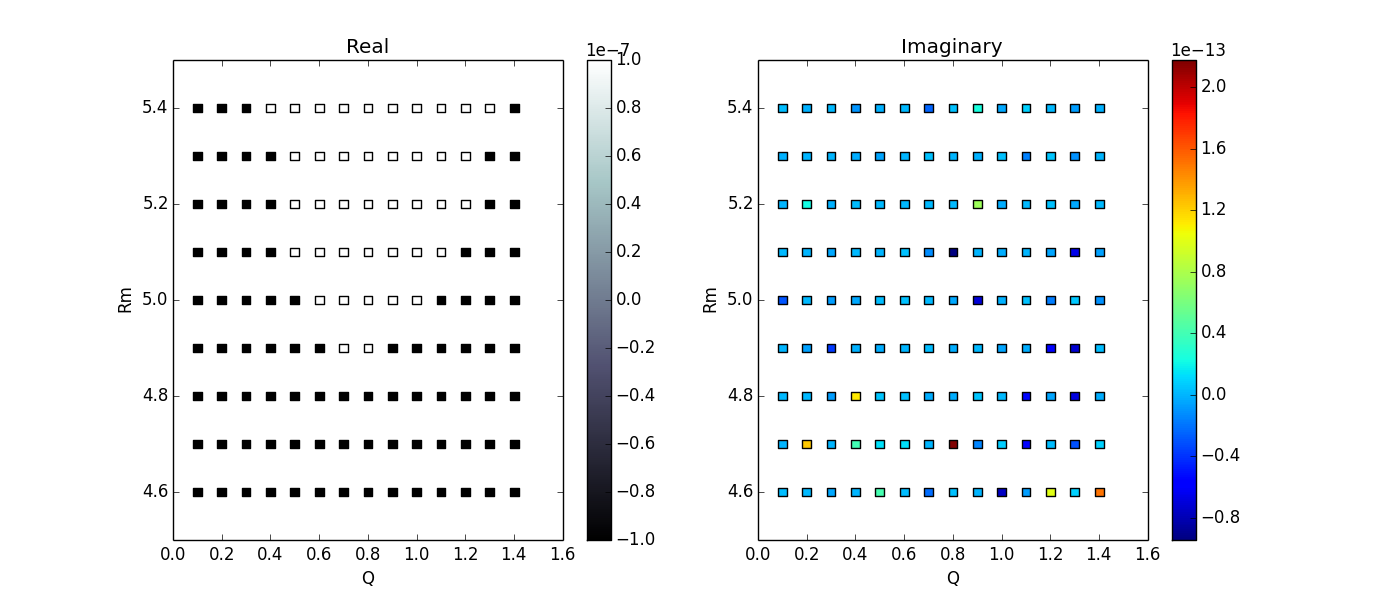
\includegraphics[width=\textwidth]{s_Re_Im_Co_coarse}
\caption{Real and Imaginary parts of parameter space for linear MRI system: coarse grid}
\end{figure*}

By solving the linear MRI system on a coarse parameter space grid. We then zoom in to find the critical values of $\reym$ and $Q$:\\

\begin{figure*}[h!]
\centering
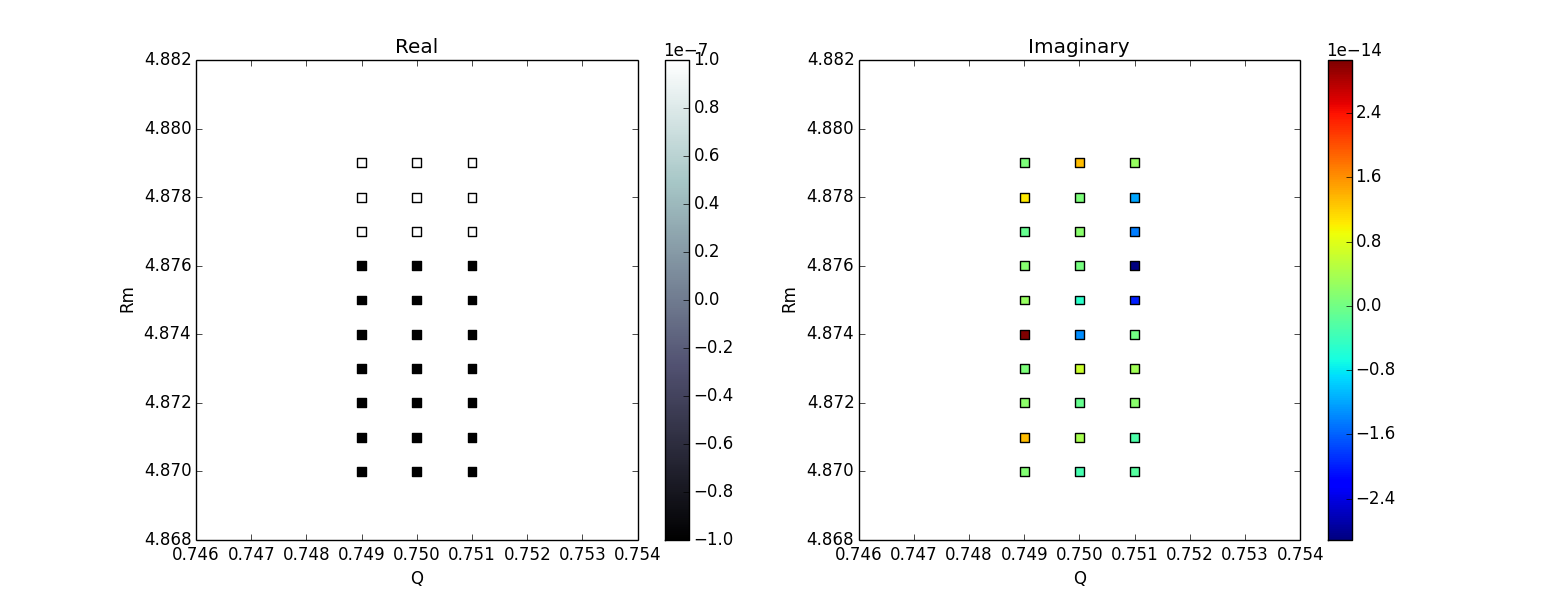
\includegraphics[width=\textwidth]{s_Re_Im_Co_finegrid3}
\caption{Real and Imaginary parts of parameter space for linear MRI system: fine grid}
\end{figure*}

The code that produces the above is in \texttt{multirun\_paramspace.py}, which runs\\ \texttt{multirun\_linear\_MRI.py}. \\

From this investigation, I have been using $Q = 0.75$, $\reym = 4.877$, rather than the $\reym \sim 4.9$ given in Umurhan+. The adjoint homogenous solution, however, still does not resemble the one found in Umurhan+. Our solution is shown in Figure \ref{AHsol}:

\begin{figure*}[h!]
\centering
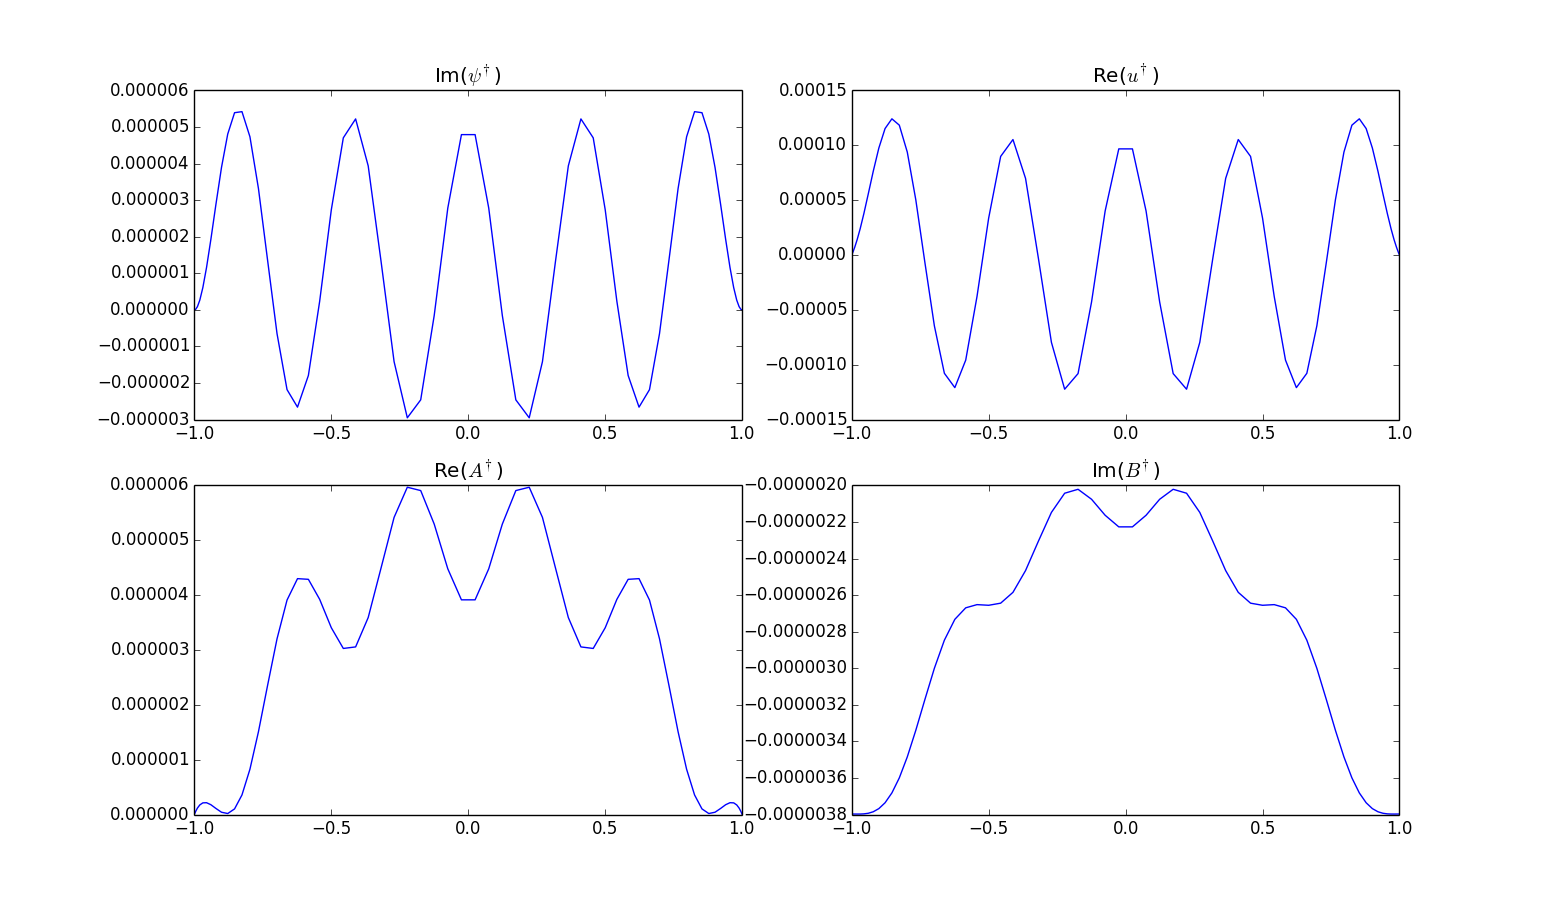
\includegraphics[width=\textwidth]{adjoint_soln_incorrect}
\caption{Adjoint homogenous solution.}
\label{AHsol}
\end{figure*}

While this solution is symmetric about the origin, as expected, it does not have the same shape as the solution in Umurhan+. Note that the normalization is arbitrary. \\

We also use Dedalus to solve the linear MRI at marginality, that is, Umurhan+ Figure 2. Our solution, which agrees with theirs, is shown in Figure \ref{margsol}:

\begin{figure*}[h!]
\centering
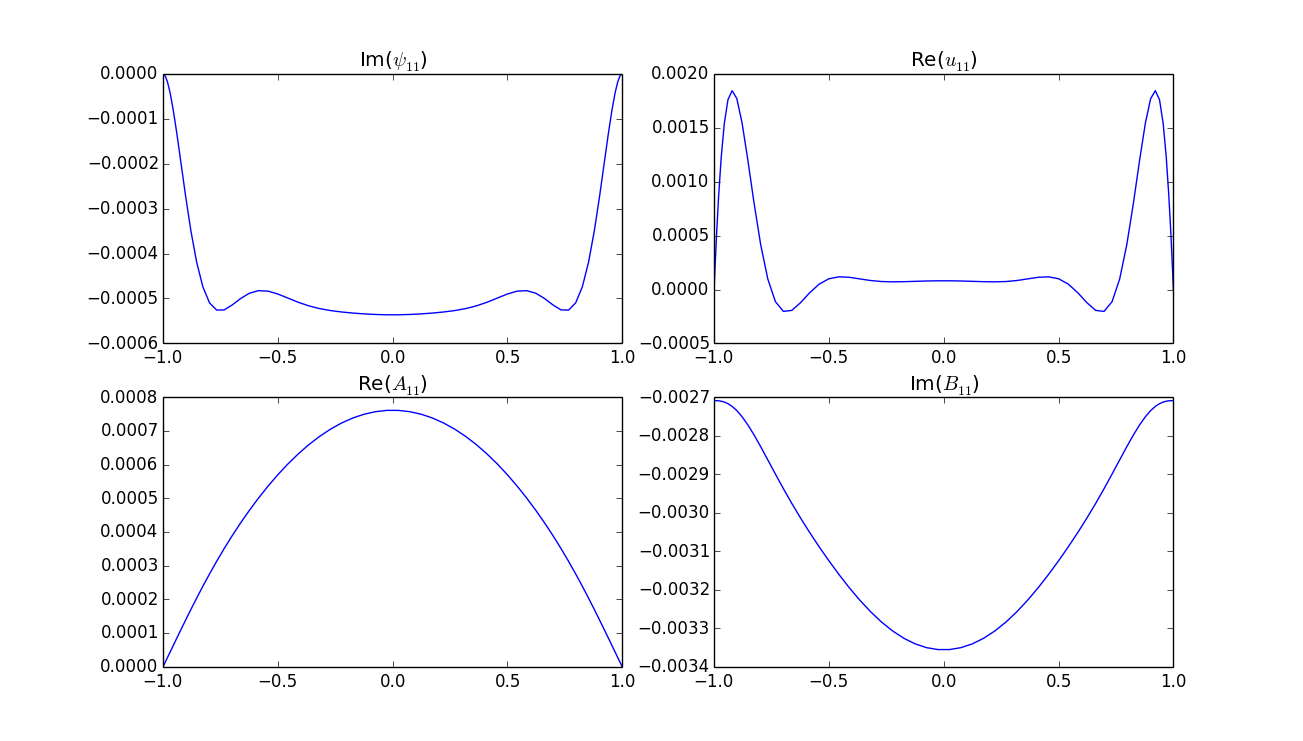
\includegraphics[width=\textwidth]{marginal_solution}
\caption{Marginal mode eigenfunctions.}
\label{margsol}
\end{figure*}

\pagebreak
The correct adjoint homogenous solution is still elusive. Here is everything I have tried so far. In what follows, red is the solution indicated in the title, and black is supposed to be zero everywhere. \\

1. $L = L_0 - L_1 dz + L_2 dz^2 - L_3 dz^3 + L_4 dz^4$ \\

Smallest eigenvalue: [-0.00624309 +1.97781664e-16j] \\

\begin{figure*}[h!]
\centering
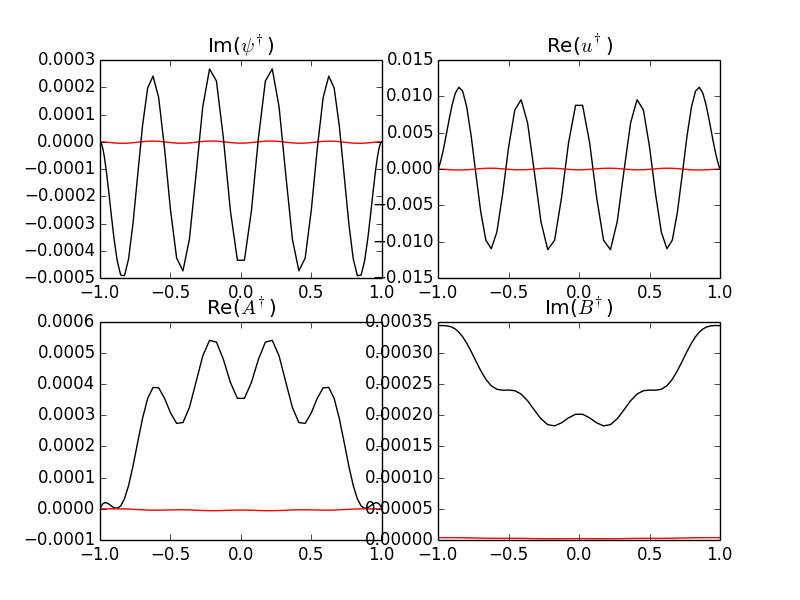
\includegraphics[scale=0.5]{ah_attempt1}
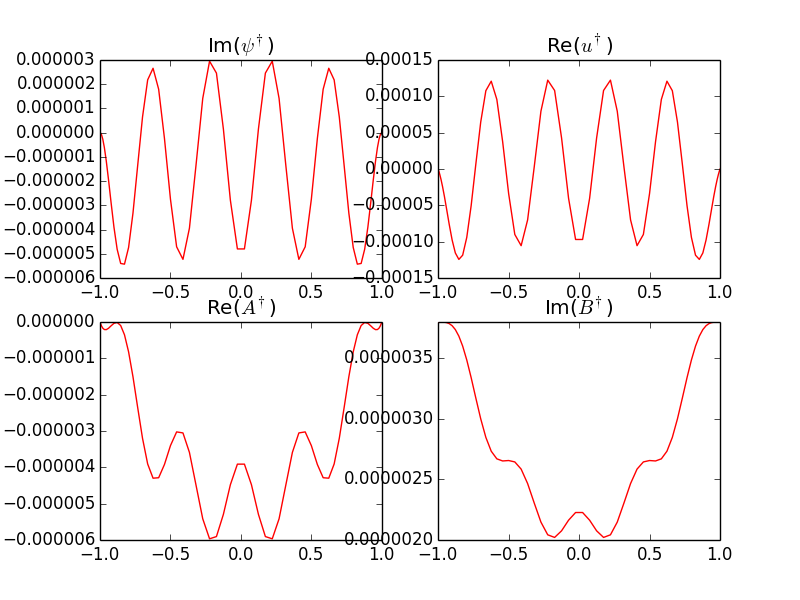
\includegraphics[scale=0.5]{ah_attempt1_redonly}
\end{figure*}

\pagebreak
2. $L = L_0 + L_1 dz - L_2 dz^2 - L_3 dz^3 + L_4 dz^4$ \\

Smallest eigenvalue: [-0.00624309 +1.97781664e-16j] \\

\begin{figure*}[h!]
\centering
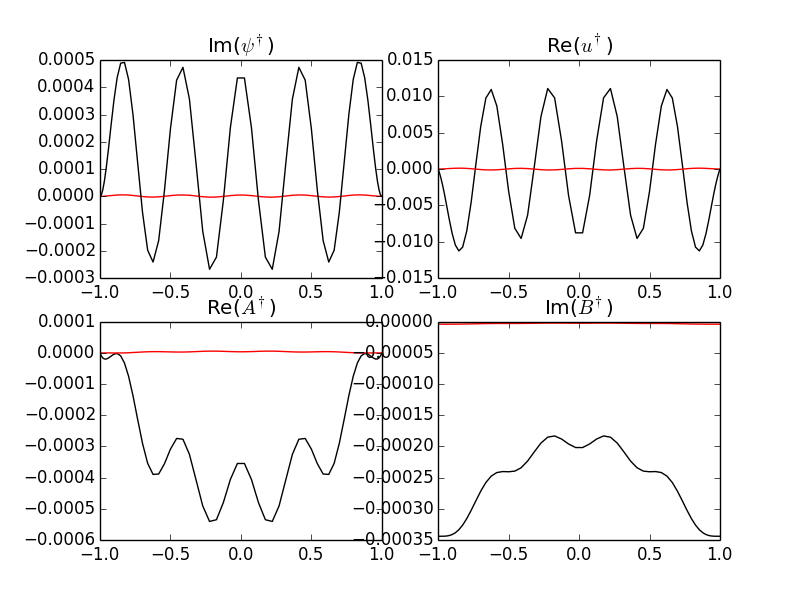
\includegraphics[scale=0.5]{ah_pmmp}
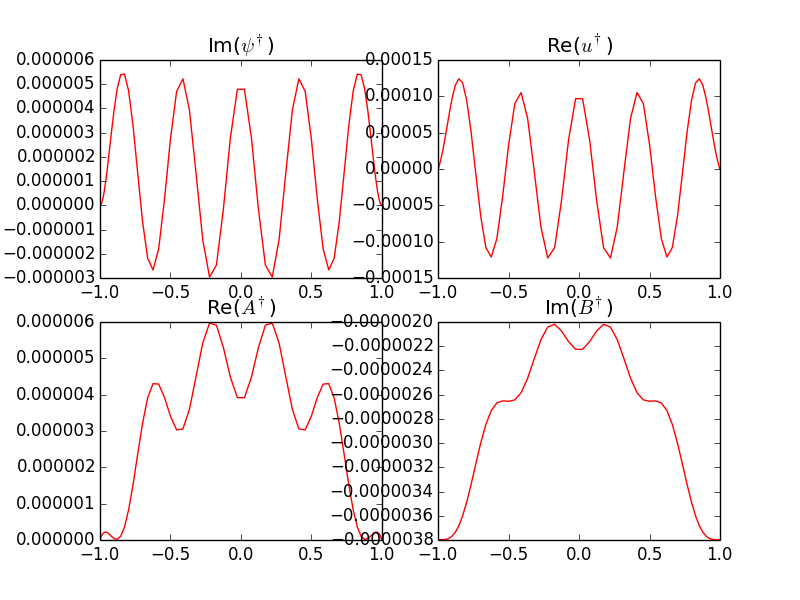
\includegraphics[scale=0.5]{ah_pmmp_redonly}
\end{figure*}

\pagebreak
3. $L = L_0 + L_1 dz + L_2 dz^2 + L_3 dz^3 + L_4 dz^4$ \\

Smallest eigenvalue: [-0.00624309 +1.97781664e-16j] \\

\begin{figure*}[h!]
\centering
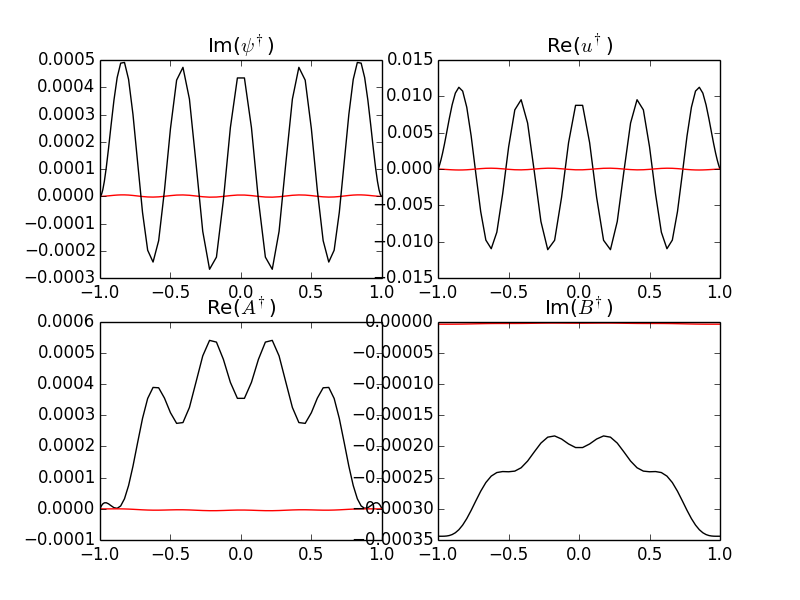
\includegraphics[scale=0.5]{ah_allpos}
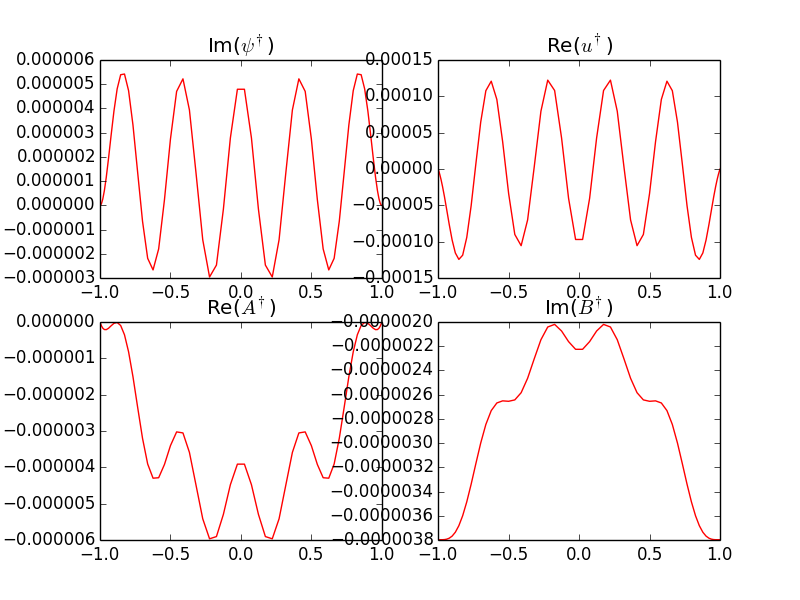
\includegraphics[scale=0.5]{ah_allpos_redonly}
\end{figure*}

\pagebreak
I also tried to solve the equations without any iQ's -- that is, without the $\partial_z$ terms: \\

\begin{figure*}[h!]
\centering
\includegraphics[scale=0.5]{ah_nodz}
\end{figure*}

And here is the solution to the *non-adjoint* $LV = 0$ equation:

\begin{figure*}[h!]
\centering
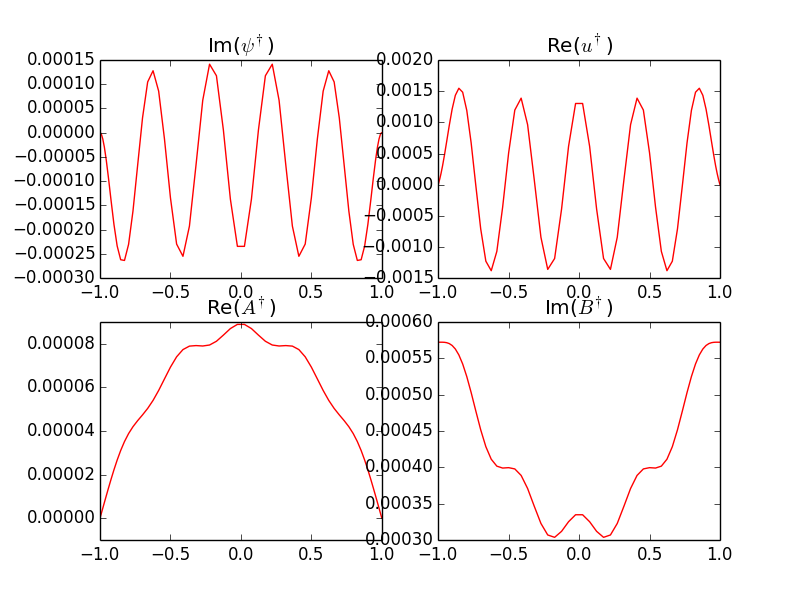
\includegraphics[scale=0.5]{nonadjoint_redonly}
\end{figure*}


Finally, the solution to the equations:

\begin{figure*}[h!]
\centering
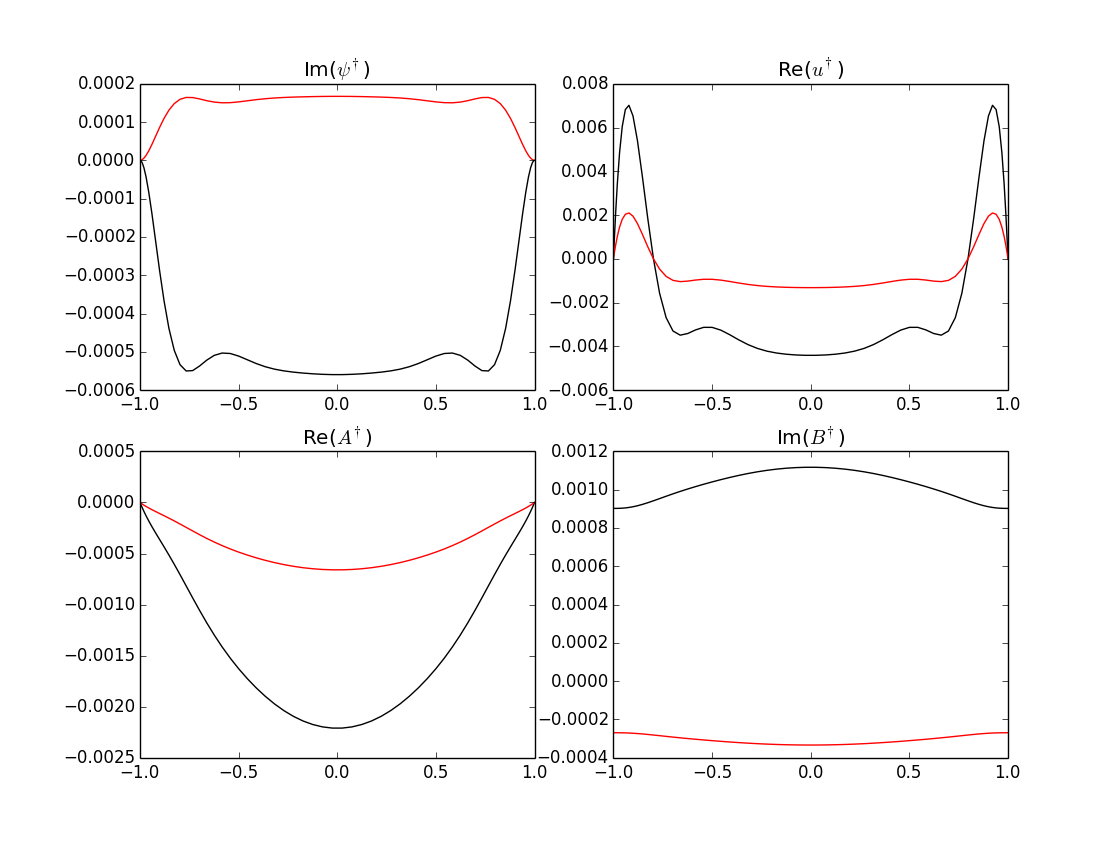
\includegraphics[scale=0.5]{ah_allpos_fixed}
\end{figure*}


\pagebreak
\section*{Helical MRI}

Instead of the standard MRI, we initialize an azimuthal field in addition to the constant vertical field. The azimuthal field will linearly decrease radially, since in any reasonable setup it will be created by an axial current through the center of the apparatus.

The base state becomes:

\begin{equation}
\mathbf{B} = B_0 \hat{z} + \xi B_0 \left(\frac{x_1}{x}\right) \hat{y} + \mathbf{B}_1
\end{equation}

The Lorentz term in the momentum equation is the only term that will change. It becomes

\beq
\left(\nabla \times \left(B_0 \hat{z} + \xi B_0 \left(\frac{x_1}{x}\right) \hat{y} + \mathbf{B}_1
\right) \right) \times \left(B_0 \hat{z} + \xi B_0 \left(\frac{x_1}{x}\right) \hat{y} + \mathbf{B}_1
\right)
\eeq

and we gain a potential 5 terms that were not present before, since there are 5 terms in this expansion that involve the azimuthal term. These are as follows.

\beq
\left(\nabla \times B_0 \hat{z} \right) \times \xi B_0 \left(\frac{x_1}{x}\right)\hat{y} = 0
\eeq

because of the constant term.

\beq
\left(\nabla \times \xi B_0 \left(\frac{x_1}{x}\right) \hat{y} \right) \times B_0 \hat{z} = \left(\partial_x \left(\xi B_0 \left(\frac{x_1}{x}\right)\right)\hat{z}\right) \times B_0 \hat{z} = 0
\eeq

because $\hat{z} \times \hat{z} = 0$.

\beq
\left(\nabla \times \xi B_0 \frac{x_1}{x} \hat{y} \right) \times \left( \xi B_0 \frac{x_1}{x}\hat{y}\right) = \xi^2 B_0^2 \frac{x_1^2}{x^3} \hat{x}
\eeq

And

\beq
\left(\nabla \times \xi B_0 \frac{x_1}{x} \hat{y}\right) \times \mathbf{B_1} = -\xi B_0 \frac{x_1}{x^2} \left(B_{1x} \hat{y} - B_{1y} \hat{x}\right)
\eeq

And finally,

\beq
\left(\nabla \times \mathbf{B}_1 \right) \times \left(\xi B_0 \frac{x_1}{x} \hat{y}\right) = - \partial_z B_{1y} \xi B_0 \frac{x_1}{x} \hat{z} - \partial_x B_{1y} \xi B_0 \frac{x_1}{x} \hat{x}
\eeq

So our final added terms to the momentum equation are:

\beq
\label{momeq_added}
\xi^2 B_0^2 \frac{x_1^2}{x^3} \hat{x} \, - \,  \xi B_0 \frac{x_1}{x^2} B_{1x} \hat{y} \, + \, \xi B_0 \frac{x_1}{x^2} B_{1y} \hat{x} \, - \, \partial_z B_{1y} \xi B_0 \frac{x_1}{x} \hat{z} \, - \, \partial_x B_{1y} \xi B_0 \frac{x_1}{x} \hat{x}
\eeq

For the induction equation, we have:

\beq
\partial_t \mathbf{B} = \left(\mathbf{B} \cdot \nabla \right) \mathbf{u} - \left(\mathbf{u} \cdot \nabla \right) \mathbf{B} + \frac{1}{\reym} \nabla^2 \mathbf{B}
\eeq

The first term on the righthand side becomes:

\beq
\left( \left( \mathbf{B_0} \hat{z} + \xi B_0 \frac{x_1}{x} \hat{y} + \mathbf{B_1} \right) \cdot \nabla \right) \left(-q \Omega_0 x \hat{y} + \mathbf{u_1}\right) = \xi B_0 \frac{x_1}{x} \partial_y \mathbf{u_1}
\eeq

The second term becomes:

\beq
-\left( \left( -q \Omega_0 x \hat{y} + \mathbf{u_1}\right) \cdot \nabla\right) \left( B_0 \hat{z} + \xi B_0 \frac{x_1}{x} \hat{y} + \mathbf{B_1}\right)   \, = \, \xi B_0 u_{1x} \frac{x_1}{x^2} \hat{y}
\eeq

And the third term on the righthandside becomes

\beq
\frac{1}{\reym} \xi B_0 \left( \frac{2 x_1}{x^3}\right) \hat{y}
\eeq

So that all told, the induction equation gains the terms:

\beq
\xi B_0 \frac{x_1}{x} \partial_y \mathbf{u_1} \, + \, \xi B_0 u_{1x} \frac{x_1}{x^2} \hat{y} \, + \, \frac{1}{\reym} \xi B_0 \left( \frac{2 x_1}{x^3}\right) \hat{y}
\eeq

Because the $\partial_y$ terms go to zero, the induction equation only picks up terms in its $y$ component (the first term above goes to zero). Rewritten to use the stream function, these terms are:

\beq
\label{induc_eq_added}
\xi B_0 \frac{x_1}{x^2} \partial_z \Psi \hat{y} + \frac{1}{\reym} \xi B_0 \frac{2 x_1}{x^3} \hat{y}
\eeq 

%We can now inspect Equation \ref{momeq_added} and see that the $\hat{y}$ component of the momentum equation will pick up a term analogous to the the first term of Equation \ref{induc_eq_added} -- a tantalizing $\partial_z$ term, which has the ability to lend a $\partial_Z$ term in the $\mathcal{O}\left(\epsilon^2\right)$ equation! But Equation \ref{momeq_added} can no longer be written in terms of flux/stream functions, because contributions to the $\hat{x}$ and $\hat{z}$ components are uneven. Should I rewrite all the equations in terms of primitive variables to proceed?

For the momentum equation, we now take $\partial_z$ of the x component and $\partial_x$ of the z component, to obtain, for each component:

\beq
[x]: \xi B_0 \frac{x_0}{x^2} \partial_z B_{1y} - \partial_x\partial_z B_{1y} \xi B_0 \frac{x_0}{x}
\eeq

\beq
[y]: - \xi B_0 \frac{x_0}{x^2} B_{1x}
\eeq

\beq
[z]: \xi B_0 \frac{x_0}{x^2} \partial_z B_{1y} - \partial_x\partial_z B_{1y} \xi B_0 \frac{x_0}{x}
\eeq

Rewritten in terms of flux functions:

\beq
[x]: \xi B_0 \frac{x_0}{x^2} \partial_z B_{y} - \partial_x\partial_z B_{y} \xi B_0 \frac{x_0}{x}
\eeq

\beq
[y]: - \xi B_0 \frac{x_0}{x^2} \partial_z A
\eeq

\beq
[z]: \xi B_0 \frac{x_0}{x^2} \partial_z B_{y} - \partial_x\partial_z B_{y} \xi B_0 \frac{x_0}{x}
\eeq

This means that the total added contributions to the final equation set, in $\left[\Psi, u_y, A, B_y\right]^T$ order, are:

\beq
[\Psi]: \xi B_0 \frac{x_0}{x^2} \partial_z B_{y} - \xi B_0 \partial_x\partial_z B_{y} \frac{x_0}{x}
\eeq

\beq
[u_y]: - \xi B_0 \frac{x_0}{x^2} \partial_z A
\eeq

\beq
[A]: 0
\eeq

\beq
[B]: \xi B_0 \frac{x_1}{x^2} \partial_z \Psi + \frac{1}{\reym} \xi B_0 \frac{2 x_1}{x^3}
\eeq

Two exciting things are happening. We have some first-order $\partial_z$ terms, and some linear coupling between the velocity and magnetic field equations.


\bibliography{mri.bib}

\end{document}